\documentclass{beamer}
\usetheme{Madrid}
\usecolortheme{default}
\usepackage[utf8]{inputenc}
\usepackage{amsmath}
\usepackage{amsfonts}
\usepackage{amssymb}
\usepackage{tikz}
\usepackage{xcolor}
\usepackage{hyperref}

\title{CRISC Exam - Hard Concepts \& Exam Traps}
\subtitle{Deep Dive Tutorial Organized by the Four CRISC Domains}
\author{CRISC Mastery Series}
\date{\today}

\begin{document}
	
	% ============================================================
	% TITLE SLIDE
	% ============================================================
	\begin{frame}
		\titlepage
	\end{frame}
	
	% ============================================================
	% OUTLINE
	% ============================================================
	\begin{frame}{Tutorial Outline}
		\tableofcontents
	\end{frame}
	
	% ============================================================
	% ============================================================
	% DOMAIN 1: IT RISK IDENTIFICATION
	% ============================================================
	% ============================================================
	
	\section{Domain 1: IT Risk Identification}
	
	% ---------- 1.0 DOMAIN 1 OVERVIEW ----------
	\begin{frame}{Domain 1 Overview: IT Risk Identification}
		\begin{block}{What This Domain Covers}
			\begin{itemize}
				\item Governance, risk culture, and accountability
				\item The three lines of defense and role confusion
				\item Risk appetite, tolerance, and capacity
				\item CIA triad and information security objectives
				\item Risk awareness and communication
				\item Enterprise and interdisciplinary risk views
				\item Legal, regulatory, and privacy obligations
				\item Enterprise architecture and frameworks
			\end{itemize}
		\end{block}
	\end{frame}
	
	% ---------- 1.1 GOVERNANCE ----------
	\begin{frame}{1.1.1 What is Governance?}
		\begin{block}{Definition}
			Governance provides \textbf{direction, oversight, and accountability} to ensure enterprise objectives are achieved and aligned with stakeholder expectations.
		\end{block}
		\begin{alertblock}{Critical Insight}
			Governance \textbf{comes before} management activities. It is the foundation that aligns risk management with business objectives.
		\end{alertblock}
	\end{frame}
	
	\begin{frame}{1.1.2 Governance vs Management}
		\begin{columns}
			\begin{column}{0.5\textwidth}
				\begin{block}{Governance}
					\begin{itemize}
						\item Provides direction
						\item Establishes accountability
						\item Aligns with stakeholder expectations
						\item Oversees performance
					\end{itemize}
				\end{block}
			\end{column}
			\begin{column}{0.5\textwidth}
				\begin{block}{Management}
					\begin{itemize}
						\item Implements controls
						\item Performs risk assessments
						\item Executes procedures
						\item Runs day-to-day operations
					\end{itemize}
				\end{block}
			\end{column}
		\end{columns}
		\begin{exampleblock}{Exam Rule}
			When the question emphasizes senior leadership, organizational objectives, and stakeholder expectations $\rightarrow$ choose \textbf{governance and accountability structures}.
		\end{exampleblock}
	\end{frame}
	
	\begin{frame}{1.1.3 Board Oversight and Direction}
		\begin{block}{Who Provides Oversight?}
			Oversight and direction are the responsibility of the \textbf{Board of Directors}.
		\end{block}
		\begin{itemize}
			\item \textbf{Management} executes, does not provide oversight
			\item \textbf{Senior staff} do not provide governance oversight
			\item \textbf{IT risk manager} executes risk activities
		\end{itemize}
		\begin{alertblock}{Exam Tip}
			Oversight = Board. Execution = Management. Assurance = Audit.
		\end{alertblock}
	\end{frame}
	
	\begin{frame}{1.1.4 First Step in IT Risk Management}
		\begin{block}{The Risk Lifecycle Starts Here}
			\textbf{IT risk identification} is the first step of IT risk management.
		\end{block}
		\begin{exampleblock}{Key Saying}
			"You cannot protect what you do not know exists."
		\end{exampleblock}
		\begin{itemize}
			\item Identification $\rightarrow$ Assessment $\rightarrow$ Response $\rightarrow$ Monitoring $\rightarrow$ Reporting
			\item Reporting is the final step
		\end{itemize}
	\end{frame}
	
	\begin{frame}{1.1.5 Policy Documentation Hierarchy}
		\begin{block}{High-Level Intent}
			The high-level intent of an organization's security practices is best established by \textbf{policies}.
		\end{block}
		\begin{tabular}{|p{3cm}|p{8cm}|}
			\hline
			\textbf{Document} & \textbf{Purpose} \\
			\hline
			Policies & Express management intent at a high level \\
			\hline
			Procedures & Detailed steps for execution \\
			\hline
			Guidelines & Recommendations \\
			\hline
			Processes & Operational workflows \\
			\hline
		\end{tabular}
	\end{frame}
	
	\begin{frame}{1.1.6 RACI Model}
		\begin{block}{RACI Roles}
			\begin{tabular}{|p{2.5cm}|p{8cm}|}
				\hline
				\textbf{Role} & \textbf{Meaning} \\
				\hline
				Responsible & Does the work \\
				\hline
				Accountable & Provides resources; ultimately answerable \\
				\hline
				Consulted & Subject matter experts; provide guidance \\
				\hline
				Informed & Kept updated \\
				\hline
			\end{tabular}
		\end{block}
		\begin{alertblock}{Exam Tip}
			When you need \textbf{expert guidance}, reach out to the \textbf{Consulted} group.
		\end{alertblock}
	\end{frame}
	
	% ---------- 1.2 RISK CULTURE ----------
	\begin{frame}{1.2.1 Understanding Risk Culture}
		\begin{block}{What is Risk Culture?}
			Risk culture represents the \textbf{shared values, attitudes, and behaviors} regarding risk management within an organization.
		\end{block}
		\begin{alertblock}{Critical Insight}
			Organizational behavior has a \textbf{greater impact} on risk management effectiveness than any framework, tool, or policy.
		\end{alertblock}
		\begin{itemize}
			\item \textbf{Healthy}: Open communication, learning from failure, proactive escalation
			\item \textbf{Toxic}: Blame, fear of reporting, hiding mistakes, finger-pointing
		\end{itemize}
	\end{frame}
	
	\begin{frame}{1.2.2 The Blame Culture Phenomenon}
		\begin{block}{How Blame Culture Destroys Risk Management}
			\begin{itemize}
				\item People \textbf{hide mistakes} rather than report them
				\item No one \textbf{speaks up} about emerging risks
				\item Issues escalate until they become \textbf{major incidents}
				\item \textbf{Accountability is destroyed} - no one takes ownership
				\item \textbf{Root causes} are never identified or addressed
				\item Business units \textbf{point fingers} at IT when projects fail
			\end{itemize}
		\end{block}
		\begin{alertblock}{Hard Truth}
			A blame culture is the \textbf{MOST effective inhibitor} of relevant and efficient communication in any organization.
		\end{alertblock}
	\end{frame}
	
	\begin{frame}{1.2.3 Why Blame Culture is Primary Concern}
		\begin{block}{Consequences of Blame Culture}
			\begin{itemize}
				\item \textbf{False sense of confidence} at top management
				\item \textbf{Perception of covering up} known risks
				\item \textbf{Misalignment} between risk appetite and policies
				\item \textbf{Inhibited communication} across all levels
				\item \textbf{Reduced risk awareness} among staff
			\end{itemize}
		\end{block}
		\begin{exampleblock}{Key Takeaway}
			Before implementing any framework, tools, or policies, the organization must establish \textbf{psychological safety}.
		\end{exampleblock}
	\end{frame}
	
	\begin{frame}{1.2.4 Overconfidence as a Culture Symptom}
		\begin{block}{The Overconfidence Trap}
			When business units believe "our teams can handle any issue without additional controls," this is a \textbf{problematic risk culture} indicator.
		\end{block}
		\begin{itemize}
			\item Overconfidence $\rightarrow$ dismissed risk findings
			\item Dismissed findings $\rightarrow$ inadequate controls
			\item Inadequate controls $\rightarrow$ underestimated exposure
		\end{itemize}
		\begin{alertblock}{Exam Clue}
			Dismissal of risk information or resistance to challenge points to a \textbf{weak risk culture}, not maturity.
		\end{alertblock}
	\end{frame}
	
	\begin{frame}{1.2.5 New Risk Manager's First Focus}
		\begin{block}{Joining an Organization with Past Incidents}
			The primary focus in the first few months should be to \textbf{understand the organization's culture toward risk}.
		\end{block}
		\begin{itemize}
			\item \textbf{Wrong}: Cite individuals who caused incidents (counterproductive)
			\item \textbf{Wrong}: Draft strategy before understanding culture
			\item \textbf{Wrong}: Complete all training first (secondary)
			\item \textbf{Correct}: Understand the risk culture first
		\end{itemize}
	\end{frame}
	
	% ---------- 1.3 THREE LINES OF DEFENSE ----------
	\begin{frame}{1.3.1 The Three Lines Model}
		\begin{block}{Three Lines of Defense}
			\begin{tabular}{|p{2cm}|p{4cm}|p{5cm}|}
				\hline
				\textbf{Line} & \textbf{Who} & \textbf{Primary Responsibility} \\
				\hline
				\textbf{1st} & Operational Management & Own and manage risk; implement controls \\
				\hline
				\textbf{2nd} & Risk Oversight Functions & Monitor, challenge, provide guidance \\
				\hline
				\textbf{3rd} & Internal Audit & Provide independent assurance \\
				\hline
			\end{tabular}
		\end{block}
		\begin{alertblock}{Critical Insight}
			Each line has \textbf{distinct, non-overlapping responsibilities}. Confusing these roles is a \textbf{major exam trap}.
		\end{alertblock}
	\end{frame}
	
	\begin{frame}{1.3.2 Third Line of Defense}
		\begin{block}{Primary Responsibility of 3rd LoD}
			\textbf{Independent assurance of controls} through internal/external audit.
		\end{block}
		\begin{itemize}
			\item \textbf{Policy development} = 2nd Line
			\item \textbf{User reviews} = 1st Line (operational)
			\item \textbf{Access control} = 1st Line (operational)
			\item \textbf{Independence} is the key characteristic of 3rd LoD
		\end{itemize}
	\end{frame}
	
	\begin{frame}{1.3.3 Common Role Confusion Traps}
		\begin{block}{Trap 1: Who Owns Risk?}
			\textbf{Wrong}: IT owns technology risk. \quad \textbf{Correct}: \textbf{Business management} owns all risk.
		\end{block}
		\begin{block}{Trap 2: Who Establishes Framework?}
			\textbf{Wrong}: Internal audit. \quad \textbf{Correct}: \textbf{Second Line} establishes and maintains framework.
		\end{block}
		\begin{exampleblock}{Memory Aid}
			\textbf{First = "Do It"} | \textbf{Second = "Watch It"} | \textbf{Third = "Check It"}
		\end{exampleblock}
	\end{frame}
	
	\begin{frame}{1.3.4 Role Responsibilities Table}
		\begin{table}
			\centering
			\begin{tabular}{|p{2.5cm}|p{3.5cm}|p{5cm}|}
				\hline
				\textbf{Role} & \textbf{Line of Defense} & \textbf{Key Responsibilities} \\
				\hline
				Risk Owner & 1st Line & Identifies, assesses, responds to risk \\
				\hline
				Control Owner & 1st Line & Implements and maintains controls \\
				\hline
				Risk Manager & 2nd Line & Monitors risk; provides oversight \\
				\hline
				CRO & 2nd Line & Oversees risk management program \\
				\hline
				Internal Audit & 3rd Line & Provides independent assurance \\
				\hline
				Board & Governance & Sets risk appetite; provides direction \\
				\hline
			\end{tabular}
		\end{table}
	\end{frame}
	
	\begin{frame}{1.3.5 Symptoms of Dysfunction}
		\begin{block}{When Lines Don't Work Together}
			\begin{itemize}
				\item \textbf{Each line planning independently} - Most dangerous sign
				\item Overlap in responsibilities causing confusion
				\item Gaps where no one takes ownership
				\item Duplicate work across lines
				\item Conflict between lines regarding authority
			\end{itemize}
		\end{block}
		\begin{alertblock}{Critical Risk}
			Without integrated lines of defense, the organization has \textbf{no integrated risk management} capability. Risks fall through the cracks.
		\end{alertblock}
	\end{frame}
	
	\begin{frame}{1.3.6 CRO Responsibility Trap}
		\begin{block}{What the CRO Actually Does}
			\begin{itemize}
				\item Manages the \textbf{risk assessment process}
				\item Ensures \textbf{corrective actions} are implemented
				\item Manages the \textbf{supporting risk management function}
				\item Provides \textbf{oversight, guidance, coordination}
			\end{itemize}
		\end{block}
		\begin{alertblock}{CRO Trap}
			Students select the CRO because the title contains "Risk." But the CRO \textbf{does not own business risk} and \textbf{does not accept risk} on behalf of the business.
		\end{alertblock}
	\end{frame}
	
	% ---------- 1.4 RISK APPETITE, TOLERANCE, CAPACITY ----------
	\begin{frame}{1.4.1 The Three Risk Concepts}
		\begin{block}{Concept Definitions}
			\begin{tabular}{|p{3cm}|p{8cm}|}
				\hline
				\textbf{Concept} & \textbf{Definition} \\
				\hline
				\textbf{Risk Appetite} & Amount of risk an organization is \textbf{willing to accept} in pursuit of its mission \\
				\hline
				\textbf{Risk Tolerance} & \textbf{Acceptable level of variation} from risk appetite for a specific risk \\
				\hline
				\textbf{Risk Capacity} & \textbf{Maximum risk} an organization can absorb before existence is threatened \\
				\hline
			\end{tabular}
		\end{block}
		\begin{alertblock}{Critical Distinction}
			\textbf{Appetite} = Willing to take | \textbf{Tolerance} = Acceptable deviation | \textbf{Capacity} = Can survive
		\end{alertblock}
	\end{frame}
	
	\begin{frame}{1.4.2 The Hierarchy Relationship}
		\begin{center}
			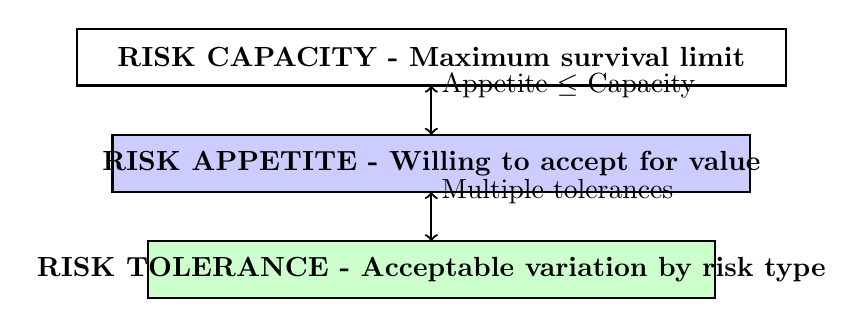
\begin{tikzpicture}[scale=0.9]
				\draw[thick] (0,0) rectangle (10,0.8) node[midway] {\textbf{RISK CAPACITY - Maximum survival limit}};
				\draw[thick, fill=blue!20] (0.5,-1.5) rectangle (9.5,-0.7) node[midway] {\textbf{RISK APPETITE - Willing to accept for value}};
				\draw[thick, fill=green!20] (1,-3) rectangle (9,-2.2) node[midway] {\textbf{RISK TOLERANCE - Acceptable variation by risk type}};
				\draw[<->, thick] (5,-2.2) -- (5,-1.5) node[right] {Multiple tolerances};
				\draw[<->, thick] (5,-0.7) -- (5,0) node[right] {Appetite $\le$ Capacity};
			\end{tikzpicture}
		\end{center}
		\begin{exampleblock}{Rule}
			Appetite is always less than or equal to Capacity.
		\end{exampleblock}
	\end{frame}
	
	\begin{frame}{1.4.3 Common Confusion Traps}
		\begin{block}{Trap 1: Appetite vs Tolerance}
			\textbf{Wrong}: Using them interchangeably. \\
			\textbf{Correct}: Appetite is \textbf{broad}; tolerance is \textbf{specific} acceptable deviation.
		\end{block}
		\begin{block}{Trap 2: Tolerance vs Capacity}
			\textbf{Wrong}: Thinking a tolerance breach is existential. \\
			\textbf{Correct}: Tolerance breach requires action; capacity breach threatens existence.
		\end{block}
		\begin{exampleblock}{Example}
			15\% project overrun = tolerance. Bankruptcy = capacity.
		\end{exampleblock}
	\end{frame}
	
	\begin{frame}{1.4.4 Risk Tolerance Example}
		\begin{block}{Scenario}
			Board approves limited operational disruptions. Management permits customer-facing systems to be unavailable no more than 2 hours per quarter before escalation.
		\end{block}
		\begin{exampleblock}{Answer}
			This threshold is \textbf{Risk Tolerance} - acceptable deviation from appetite translated into a measurable limit.
		\end{exampleblock}
		\begin{itemize}
			\item Risk Capacity = maximum survivable risk
			\item Risk Avoidance = eliminating the activity
			\item Risk Transfer = shifting financial impact
		\end{itemize}
	\end{frame}
	
	\begin{frame}{1.4.5 Why Appetite Aligns with Business Objectives}
		\begin{block}{Purpose of Alignment}
			Risk appetite aligned with business objectives allows the enterprise to \textbf{evaluate and deploy valuable resources toward objectives where risk tolerance is low}.
		\end{block}
		\begin{alertblock}{Common Wrong Answers}
			\begin{itemize}
				\item "Major risk is identified and eliminated" - Risk elimination is rarely cost-effective
				\item "IT and business goals are aligned" - Too narrow; appetite spans the enterprise
				\item "Risk strategy is adequately communicated" - Communication doesn't depend on alignment
			\end{itemize}
		\end{alertblock}
		\begin{exampleblock}{Chain}
			Strategy Drives Appetite $\rightarrow$ Appetite Drives Investment $\rightarrow$ Investment Drives Controls
		\end{exampleblock}
	\end{frame}
	
	\begin{frame}{1.4.6 Two Major Factors for Risk Appetite}
		\begin{block}{Deciding Risk Appetite}
			\begin{itemize}
				\item \textbf{Capacity to absorb loss} - how much can we survive?
				\item \textbf{Culture toward risk taking} - how much loss do we \textit{want} to accept?
			\end{itemize}
		\end{block}
		\begin{alertblock}{Exam Trap}
			"Risk-aware decisions" and "alignment with risk culture" are secondary or outcomes - not the primary factors.
		\end{alertblock}
	\end{frame}
	
	% ---------- 1.5 CIA TRIAD ----------
	\begin{frame}{1.5.1 Understanding CIA}
		\begin{block}{Confidentiality, Integrity, Availability}
			\begin{tabular}{|p{2.5cm}|p{4cm}|p{4.5cm}|}
				\hline
				\textbf{Principle} & \textbf{Definition} & \textbf{Example Breach} \\
				\hline
				Confidentiality & Accessible to authorized only & Disclosed to unauthorized party \\
				\hline
				Integrity & Accurate and complete & Modified by unauthorized user \\
				\hline
				Availability & Accessible when needed & Unavailable when needed \\
				\hline
			\end{tabular}
		\end{block}
		\begin{alertblock}{Critical Insight}
			There are \textbf{always trade-offs}. You cannot maximize all three simultaneously.
		\end{alertblock}
	\end{frame}
	
	\begin{frame}{1.5.2 Resilient Business Processes}
		\begin{block}{Resilience and Availability}
			Resilience = ability to \textbf{provide and maintain an acceptable level of service} during disasters or operational challenges.
		\end{block}
		\begin{exampleblock}{Correct Answer Pattern}
			Resilience questions $\rightarrow$ choose \textbf{Availability}.
		\end{exampleblock}
		\begin{itemize}
			\item Effectiveness = relevant, timely information
			\item Confidentiality = no unauthorized disclosure
			\item Integrity = accuracy and completeness
			\item Availability = accessible when required (linked to resilience)
		\end{itemize}
	\end{frame}
	
	\begin{frame}{1.5.3 Weather Forecast System}
		\begin{block}{Highest Priority: Integrity}
			A public weather forecast system places its highest priority on the \textbf{integrity of data}.
		\end{block}
		\begin{itemize}
			\item Nonrepudiation - unlikely to be important
			\item Confidentiality - at odds with public consumption
			\item Availability - important, but incorrect data may be worse than an outage
		\end{itemize}
		\begin{exampleblock}{Distinction}
			Whether the forecast is \textit{accurate in prediction} is distinct from whether the data was \textit{accurately represented}.
		\end{exampleblock}
	\end{frame}
	
	\begin{frame}{1.5.4 Business System Priority Map}
		\begin{block}{Highest Priority by System Type}
			\begin{tabular}{|p{5cm}|p{3.5cm}|}
				\hline
				\textbf{System} & \textbf{Highest Priority} \\
				\hline
				Weather forecast (public) & Integrity \\
				\hline
				Emergency services / hospital & Availability \\
				\hline
				Medical records & Confidentiality + Integrity \\
				\hline
				Contracts / digital signatures & Nonrepudiation \\
				\hline
				Resilient business processes & Availability \\
				\hline
			\end{tabular}
		\end{block}
	\end{frame}
	
	\begin{frame}{1.5.5 Confidentiality Breach Recognition}
		\begin{block}{What is a Breach of Confidentiality?}
			Improper disclosure of information to a recipient \textbf{not authorized access by the information owner}.
		\end{block}
		\begin{itemize}
			\item Data modified by unauthorized user = \textbf{Integrity}
			\item Data unavailable when needed = \textbf{Availability}
			\item Data disclosed to unauthorized recipient = \textbf{Confidentiality}
			\item Data destroyed = \textbf{Integrity/Availability}
		\end{itemize}
		\begin{exampleblock}{Scenario}
			Payroll employee emails salaries and SSNs to an external vendor with no business need $\rightarrow$ \textbf{Confidentiality} violated.
		\end{exampleblock}
	\end{frame}
	
	\begin{frame}{1.5.6 Integrity Breach Recognition}
		\begin{block}{Loss of Integrity Events}
			\begin{itemize}
				\item Unauthorized changes to a website
				\item Email message modified in transit
				\item Virus infects a file
			\end{itemize}
		\end{block}
		\begin{alertblock}{Not Integrity}
			"Someone sees the company's secret formula" = \textbf{Confidentiality} breach.
		\end{alertblock}
	\end{frame}
	
	\begin{frame}{1.5.7 Increasing Confidentiality Trade-off}
		\begin{block}{Confidentiality vs Availability}
			Increasing confidentiality typically \textbf{increases processing time and may reduce availability}.
		\end{block}
		\begin{itemize}
			\item Wrong: Increases availability
			\item Wrong: Decreases processing time
			\item Wrong: Has no effect on availability
		\end{itemize}
		\begin{exampleblock}{Exam Rule}
			CIA is about balance - not maximizing a single principle.
		\end{exampleblock}
	\end{frame}
	
	\begin{frame}{1.5.8 Balance, Not Maximum Security}
		\begin{block}{The CIA Balance Principle}
			Effective risk management balances confidentiality, integrity, and availability to \textbf{support business objectives}. Increasing one may affect another.
		\end{block}
		\begin{itemize}
			\item \textbf{Wrong}: "Confidentiality should always take precedence"
			\item \textbf{Wrong}: "Availability should always take precedence"
			\item \textbf{Wrong}: "Avoid controls that affect usability"
			\item \textbf{Correct}: Balance controls with business requirements
		\end{itemize}
		\begin{exampleblock}{Exam Rule}
			Business Objective $\rightarrow$ Risk Appetite $\rightarrow$ Security Controls $\rightarrow$ CIA Trade-offs
		\end{exampleblock}
	\end{frame}
	
	\begin{frame}{1.5.9 Weak Passwords and Unprotected Transmission}
		\begin{block}{Vulnerabilities, Not Threats}
			Weak passwords and transmission over unprotected communication lines are \textbf{vulnerabilities}.
		\end{block}
		\begin{itemize}
			\item \textbf{Vulnerability} = characteristic that may be exploited by a threat
			\item \textbf{Threat} = circumstance with potential to cause harm
			\item \textbf{Probability} = likelihood of occurrence
			\item \textbf{Impact} = outcome of threat exploiting vulnerability
		\end{itemize}
	\end{frame}
	
	\begin{frame}{1.5.10 Lack of Adequate Controls}
		\begin{block}{Vulnerability Definition}
			A \textbf{vulnerability} is a weakness or lack of safeguard that can be exploited by a threat.
		\end{block}
		\begin{itemize}
			\item Threat = potential cause of harm
			\item Asset = economic resource
			\item Impact = financial loss measure
		\end{itemize}
		\begin{exampleblock}{Exam Rule}
			"No adequate controls" $\rightarrow$ \textbf{Vulnerability}.
		\end{exampleblock}
	\end{frame}
	
	% ---------- 1.6 RISK AWARENESS & COMMUNICATION ----------
	\begin{frame}{1.6.1 IT Risk Awareness Program}
		\begin{block}{Primary Consideration}
			When developing an IT risk awareness program, the primary consideration is \textbf{how technology risk can impact each attendee's area of business}.
		\end{block}
		\begin{itemize}
			\item \textbf{Wrong}: "Why technology risk is owned by IT" - IT does NOT own technology risk
			\item \textbf{Wrong}: "How to transfer technology risk" - Transfer is a response, not awareness
			\item \textbf{Wrong}: "Why risk is more difficult to manage" - Difficulty is secondary
		\end{itemize}
	\end{frame}
	
	\begin{frame}{1.6.2 Security Awareness Training Goal}
		\begin{block}{Most Important Aspect}
			The most important aspect of security awareness training is to \textbf{create a security-conscious culture}.
		\end{block}
		\begin{itemize}
			\item Latest threats change constantly
			\item Compliance is secondary
			\item Upskilling is secondary
		\end{itemize}
	\end{frame}
	
	\begin{frame}{1.6.3 Risk Communication Defined}
		\begin{block}{Definition}
			Risk communication is the "process of \textbf{exchanging information and views about risks} among stakeholders."
		\end{block}
		\begin{itemize}
			\item Governance = decision-making structures
			\item Identification = discovering risks
			\item Response planning = mitigation actions
			\item Communication = information exchange
		\end{itemize}
	\end{frame}
	
	\begin{frame}{1.6.4 Lessons Learned Database}
		\begin{block}{After Project Completion}
			Risk responses identified during monitoring and controlling should be included in the organization's \textbf{lessons learned database}.
		\end{block}
		\begin{itemize}
			\item Project management plan is for current project execution
			\item Risk management plan is current project methodology
			\item Risk register alone doesn't share knowledge across projects
		\end{itemize}
		\begin{exampleblock}{Why?}
			Knowledge sharing benefits future projects.
		\end{exampleblock}
	\end{frame}
	
	\begin{frame}{1.6.5 Communications Management Plan}
		\begin{block}{Who Shares Risk Information?}
			The \textbf{Communications Management Plan} defines who will be available to share information on risks and responses.
		\end{block}
		\begin{itemize}
			\item Risk Management Plan - defines identification/analysis
			\item Stakeholder Management Strategy - doesn't address risk communications
			\item Resource Management Plan - doesn't define risk communications
		\end{itemize}
	\end{frame}
	
	% ---------- 1.7 ENTERPRISE & INTERDISCIPLINARY VIEWS ----------
	\begin{frame}{1.7.1 Best View of Risk Management}
		\begin{block}{Interdisciplinary Team}
			An \textbf{interdisciplinary team} provides the BEST view of risk management, ensuring all areas are adequately considered.
		\end{block}
		\begin{itemize}
			\item Third-party assessment - lacks internal knowledge
			\item IT department - doesn't reflect the entire enterprise
			\item Compliance department - focuses on regulatory implications
		\end{itemize}
	\end{frame}
	
	\begin{frame}{1.7.2 Enterprise Risk View}
		\begin{block}{Multiple Stakeholder Perspectives}
			Enterprise risk = multiple perspectives. Cross-functional team = enterprise view.
		\end{block}
		\begin{itemize}
			\item IT view = technology risk
			\item Compliance view = regulatory risk
			\item Third-party = independent view
			\item Cross-functional team = \textbf{enterprise view}
		\end{itemize}
		\begin{exampleblock}{Exam Rule}
			When CRISC asks for the BEST enterprise-wide view, choose the answer involving \textbf{multiple stakeholders}.
		\end{exampleblock}
	\end{frame}
	
	\begin{frame}{1.7.3 Business Management Accountability}
		\begin{block}{Who Analyzes Risks and Maintains Risk Profile?}
			\textbf{Business management} is accountable for analyzing risks, maintaining the risk profile, and making risk-aware decisions.
		\end{block}
		\begin{itemize}
			\item Business process owner - responsible, not accountable
			\item CIO - some responsibility, not accountability
			\item CRO - oversight, not direct accountability
		\end{itemize}
	\end{frame}
	
	\begin{frame}{1.7.4 Risk Owner Purpose}
		\begin{block}{Why Have a Risk Owner?}
			The primary reason for a risk owner is to \textbf{ensure accountability} for managing the risk.
		\end{block}
		\begin{itemize}
			\item Leveraging resources is secondary
			\item Flexibility is not the purpose
			\item Seeking assistance is secondary
		\end{itemize}
		\begin{alertblock}{Governance Rule}
			Responsibility can be delegated. \textbf{Accountability cannot.}
		\end{alertblock}
	\end{frame}
	
	% ---------- 1.8 LEGAL, REGULATORY, PRIVACY ----------
	\begin{frame}{1.8.1 Key Regulations Overview}
		\begin{block}{Major Compliance Frameworks}
			\begin{tabular}{|p{2.5cm}|p{4cm}|p{4.5cm}|}
				\hline
				\textbf{Regulation} & \textbf{Jurisdiction} & \textbf{Applies To} \\
				\hline
				HIPAA & US Federal & Health information \\
				\hline
				GDPR & EU & Personal data of EU residents \\
				\hline
				CCPA & California & Personal data of CA residents \\
				\hline
				SOX & US Federal & Public company financial reporting \\
				\hline
				PCI DSS & Global & Payment card data \\
				\hline
			\end{tabular}
		\end{block}
	\end{frame}
	
	\begin{frame}{1.8.2 HIPAA and CCPA}
		\begin{block}{HIPAA}
			Federal law protecting sensitive \textbf{health information}.
		\end{block}
		\begin{block}{CCPA}
			California law protecting \textbf{California residents' personal information}.
		\end{block}
		\begin{itemize}
			\item GDPR - EU residents
			\item PIPEDA - Canada residents
			\item FFIEC - banking regulation
		\end{itemize}
	\end{frame}
	
	\begin{frame}{1.8.3 SOX Section 302 vs 404}
		\begin{block}{Sarbanes-Oxley Key Sections}
			\begin{tabular}{|p{2cm}|p{4cm}|p{5cm}|}
				\hline
				\textbf{Section} & \textbf{Requirement} & \textbf{Key Point} \\
				\hline
				302 & CEO/CFO certification & Financial reports certified \\
				\hline
				404 & Internal controls assessment & Annual control assessment \\
				\hline
				203 & Audit partner rotation & Every 5 years \\
				\hline
				409 & Timely reporting & Real-time disclosure \\
				\hline
			\end{tabular}
		\end{block}
		\begin{alertblock}{Trap}
			Section 302 = \textbf{Certification} | Section 404 = \textbf{Controls}
		\end{alertblock}
	\end{frame}
	
	\begin{frame}{1.8.4 Regulatory Change Response}
		\begin{block}{New Law Enacted? Follow This Order}
			New Law $\rightarrow$ \textbf{Impact Assessment} $\rightarrow$ Gap Analysis $\rightarrow$ Policy/Control Updates $\rightarrow$ Implementation
		\end{block}
		\begin{alertblock}{First-Step Trap}
			\begin{itemize}
				\item Wrong: Immediately update all policies
				\item Wrong: Direct system owners to implement controls
				\item Wrong: Wait until the next review cycle
				\item Correct: Assess the impact on business processes and existing controls
			\end{itemize}
		\end{alertblock}
	\end{frame}
	
	\begin{frame}{1.8.5 Policy Exception Governance}
		\begin{block}{After an Exception Is Approved}
			Approved exceptions must be \textbf{periodically reviewed} to confirm they remain necessary, justified, and within risk appetite.
		\end{block}
		\begin{itemize}
			\item Approval does not eliminate oversight
			\item Compensating controls must remain in place
			\item Risk ownership stays with the organization
		\end{itemize}
		\begin{alertblock}{Exam Rule}
			"Exception" $\rightarrow$ approval, documentation, compensating controls, risk owner, expiration date, \textbf{periodic review}.
		\end{alertblock}
	\end{frame}
	
	\begin{frame}{1.8.6 Data Security vs Data Privacy}
		\begin{block}{Key Distinction}
			\begin{itemize}
				\item \textbf{Security} = Protect the data (encryption, firewalls, access control)
				\item \textbf{Privacy} = Use the data properly (consent, lawful basis, minimization)
			\end{itemize}
		\end{block}
		\begin{alertblock}{Classic Scenario}
			A bank encrypts records, restricts access, and monitors access attempts - but collects \textbf{more personal information than necessary}.
			
			\textbf{Conclusion}: Strong security does \textbf{not} guarantee privacy.
		\end{alertblock}
	\end{frame}
	
	\begin{frame}{1.8.7 Privacy Compliance: Consent First}
		\begin{block}{Using Personal Data for Marketing}
			Obtaining \textbf{appropriate customer consent} is the most important action to reduce privacy compliance risk.
		\end{block}
		\begin{itemize}
			\item Encryption = security, not lawful basis
			\item Firewalls = security, not lawful basis
			\item Training = supports awareness, not consent
		\end{itemize}
		\begin{exampleblock}{Memory Aid}
			You can have security without privacy. You \textbf{cannot} have privacy without security.
		\end{exampleblock}
	\end{frame}
	
	% ---------- 1.9 ENTERPRISE ARCHITECTURE ----------
	\begin{frame}{1.9.1 Architecture Components}
		\begin{block}{Four Architecture Domains}
			\begin{tabular}{|p{2.5cm}|p{4cm}|p{4.5cm}|}
				\hline
				\textbf{Domain} & \textbf{Covers} & \textbf{Components} \\
				\hline
				Business & Strategy and processes & Organization, capabilities \\
				\hline
				Application & Software solutions & Applications, APIs \\
				\hline
				Data & Data management & Models, databases, flows \\
				\hline
				Technology & Infrastructure & Network, servers, storage \\
				\hline
			\end{tabular}
		\end{block}
		\begin{alertblock}{Critical Insight}
			Technology Architecture includes \textbf{networking devices, storage, and software}.
		\end{alertblock}
	\end{frame}
	
	\begin{frame}{1.9.2 Cloud Deployment Models}
		\begin{block}{Four Cloud Deployment Models}
			\begin{tabular}{|p{2cm}|p{4.5cm}|p{4.5cm}|}
				\hline
				\textbf{Model} & \textbf{Description} & \textbf{Use Case} \\
				\hline
				Public & Shared by general public & SaaS, broad access \\
				\hline
				Private & Dedicated to one organization & High security \\
				\hline
				Community & Shared by similar organizations & Research consortium \\
				\hline
				Hybrid & Combination of models & Cloud bursting \\
				\hline
			\end{tabular}
		\end{block}
		\begin{exampleblock}{Scenario}
			Collaborative research between universities = \textbf{Community Cloud}.
		\end{exampleblock}
	\end{frame}
	
	\begin{frame}{1.9.3 Cloud Service Models}
		\begin{block}{IaaS vs PaaS vs SaaS}
			\begin{tabular}{|p{2cm}|p{5cm}|p{4cm}|}
				\hline
				\textbf{Model} & \textbf{Provides} & \textbf{Example} \\
				\hline
				IaaS & Compute, network, storage & Virtual servers \\
				\hline
				PaaS & Development platform & App hosting \\
				\hline
				SaaS & Ready-to-use software & Online game platform \\
				\hline
			\end{tabular}
		\end{block}
		\begin{alertblock}{Trap}
			Online gaming platform with no installation = \textbf{SaaS}.
		\end{alertblock}
	\end{frame}
	
	\begin{frame}{1.9.4 Architecture Frameworks}
		\begin{block}{Frameworks to Remember}
			\begin{tabular}{|p{3cm}|p{8cm}|}
				\hline
				\textbf{Framework} & \textbf{Purpose} \\
				\hline
				COBIT & IT governance \\
				\hline
				COSO ERM & Enterprise risk management \\
				\hline
				FAIR & Quantitative risk analysis \\
				\hline
				SABSA & Business-driven security architecture \\
				\hline
				Zachman & Enterprise architecture taxonomy \\
				\hline
				OCTAVE & Asset-centric risk assessment \\
				\hline
				TOGAF & Enterprise architecture method \\
				\hline
			\end{tabular}
		\end{block}
	\end{frame}
	
	\begin{frame}{1.9.5 EA Tool Traps}
		\begin{block}{Zachman Perspectives}
			Planner, Owner, Designer, Builder, Subcontractor, Functioning Enterprise. \\
			\textbf{Trap}: "Incident Manager" is NOT a Zachman perspective.
		\end{block}
		\begin{block}{Federal Enterprise Architecture}
			Promotes \textbf{alignment between business and technology}.
		\end{block}
		\begin{block}{SABSA Layers}
			Contextual, Conceptual, Logical, Physical, Component, Operational.
		\end{block}
	\end{frame}
	
	% ---------- 1.10 OTHER DOMAIN 1 CONCEPTS ----------
	\begin{frame}{1.10.1 CIA Triad as Access Control Principles}
		\begin{block}{Three Principles of Access Controls}
			Confidentiality, Integrity, and Availability.
		\end{block}
		\begin{itemize}
			\item Reliability is NOT a CIA principle
			\item Access controls support all three elements of CIA
		\end{itemize}
	\end{frame}
	
	\begin{frame}{1.10.2 Procedural Safeguards}
		\begin{block}{What are Procedural Safeguards?}
			Procedural safeguards are \textbf{administrative controls} that include:
			\begin{itemize}
				\item Policies and procedures
				\item Standards and guidelines
				\item Training and awareness
				\item Background checks and separation of duties
			\end{itemize}
		\end{block}
	\end{frame}
	
	\begin{frame}{1.10.3 Risk Utility}
		\begin{block}{Definition of Risk Utility}
			Risk utility describes the \textbf{usefulness of a particular risk to an individual or group}.
		\end{block}
		\begin{itemize}
			\item Not the finance incentive
			\item Not the potential opportunity
			\item Not the mechanics of how risk works
		\end{itemize}
	\end{frame}
	
	\begin{frame}{1.10.4 Categorizing Risks by Cause}
		\begin{block}{Primary Advantage of Grouping by Cause}
			Grouping risks by common causes assists in \textbf{developing effective risk responses}.
		\end{block}
		\begin{itemize}
			\item Related risks often have common causal factors
			\item A single response can address multiple risks
			\item Realizing areas most laden with risks is a byproduct, not primary advantage
		\end{itemize}
	\end{frame}
	
	\begin{frame}{1.10.5 Risk Maturity Level Overview (Domain 1 Context)}
		\begin{block}{Capability Maturity Model (CMM)}
			\begin{tabular}{|p{1.2cm}|p{3cm}|p{6.5cm}|}
				\hline
				\textbf{Level} & \textbf{Name} & \textbf{Characteristics} \\
				\hline
				0 & Incomplete & No risk awareness; decisions lack credible info \\
				\hline
				1 & Initial & Ad hoc; risk viewed as technical; episodic \\
				\hline
				2 & Repeatable & Basic processes; risk viewed as IT business issue \\
				\hline
				3 & Defined & Standardized; risk viewed as business issue \\
				\hline
				4 & Managed & Quantitative metrics; integrated with ERM \\
				\hline
				5 & Optimized & Real-time monitoring; continuous improvement \\
				\hline
			\end{tabular}
		\end{block}
	\end{frame}
	
	\begin{frame}{1.10.6 Level 0 vs Level 1}
		\begin{block}{Level 0 - Incomplete}
			\begin{itemize}
				\item Enterprise does \textbf{not recognize} the need for risk management
				\item Decisions involving risk \textbf{lack credible information}
			\end{itemize}
		\end{block}
		\begin{block}{Level 1 - Initial}
			\begin{itemize}
				\item Risk is recognized but treated as a \textbf{technical} issue
				\item Risk management skills exist on an ad hoc basis
				\item Risk appetite applied only during episodic assessments
			\end{itemize}
		\end{block}
		\begin{alertblock}{Trap}
			"Decisions lack credible information" = \textbf{Level 0}, NOT Level 1.
		\end{alertblock}
	\end{frame}
	
	\begin{frame}{1.10.7 Level 3 and Level 5}
		\begin{block}{Level 3 - Defined}
			\begin{itemize}
				\item Risk is a business issue
				\item Business understands IT's place in enterprise risk universe
				\item Workflow tools used
				\item Standardized processes
			\end{itemize}
		\end{block}
		\begin{block}{Level 5 - Optimized}
			\begin{itemize}
				\item Real-time monitoring of risk events
				\item Automation of policy management
				\item Formal continuous improvement
			\end{itemize}
		\end{block}
	\end{frame}
	
	\begin{frame}{1.10.8 Maturity Level Recognition Clues}
		\begin{block}{Map the Wording to the Level}
			\begin{tabular}{|p{7cm}|p{2.5cm}|}
				\hline
				\textbf{If the question says...} & \textbf{Level} \\
				\hline
				"Continuous improvement," "optimized," "real-time automation" & Level 5 \\
				\hline
				"Quantitative metrics," "integrated with ERM" & Level 4 \\
				\hline
				"Defined processes," "workflow tools," "business issue" & Level 3 \\
				\hline
				"Ad hoc," "episodic," "risk viewed as technical" & Level 1 \\
				\hline
				"Decisions lack credible information" & Level 0 \\
				\hline
			\end{tabular}
		\end{block}
	\end{frame}
	
	\begin{frame}{1.10.9 Level 3 NOT Characteristics}
		\begin{block}{What Level 3 Does NOT Include}
			\textbf{Heavy reliance on individual effort} is characteristic of lower maturity levels, not Level 3.
		\end{block}
		\begin{itemize}
			\item Level 3: Standardized, documented, communicated processes
			\item Level 3: Processes understood by personnel
			\item NOT Level 3: Ad hoc or individual-dependent processes
		\end{itemize}
		\begin{alertblock}{Exam Tip}
			"Continuous improvement" = Level 5. "Individual effort dependence" = low maturity.
		\end{alertblock}
	\end{frame}
	
	% ============================================================
	% ============================================================
	% DOMAIN 2: IT RISK ASSESSMENT
	% ============================================================
	% ============================================================
	
	\section{Domain 2: IT Risk Assessment}
	
	% ---------- 2.0 DOMAIN 2 OVERVIEW ----------
	\begin{frame}{Domain 2 Overview: IT Risk Assessment}
		\begin{block}{What This Domain Covers}
			\begin{itemize}
				\item Qualitative vs quantitative risk analysis
				\item Risk scenario development and analysis
				\item Risk ownership and assessment governance
				\item Periodic risk assessments and gap analysis
				\item Statistical methods and analysis tools
				\item Business Impact Analysis (BIA) and recovery objectives
				\item Inherent, residual, and current risk
				\item Risk register as the assessment output
			\end{itemize}
		\end{block}
	\end{frame}
	
	% ---------- 2.1 QUALITATIVE VS QUANTITATIVE ----------
	\begin{frame}{2.1.1 Analysis Methods Comparison}
		\begin{block}{Qualitative Risk Analysis}
			\begin{itemize}
				\item \textbf{Approach}: Subjective, judgment-based
				\item \textbf{Scale}: High/Medium/Low or 1-5 ratings
				\item \textbf{Cost}: Less expensive, faster
				\item \textbf{Output}: Risk ranking, priority list
				\item \textbf{Best For}: Initial screening, where data is scarce
			\end{itemize}
		\end{block}
		\begin{block}{Quantitative Risk Analysis}
			\begin{itemize}
				\item \textbf{Approach}: Statistical, data-driven
				\item \textbf{Scale}: Monetary values, percentages
				\item \textbf{Cost}: More expensive, complex
				\item \textbf{Output}: ALE, ROI, probability distributions
				\item \textbf{Best For}: High-stakes decisions, where data exists
			\end{itemize}
		\end{block}
	\end{frame}
	
	\begin{frame}{2.1.2 Quantitative Analysis Drawback}
		\begin{block}{Most Significant Drawback}
			The most significant drawback of quantitative risk analysis vs. qualitative is \textbf{higher cost}.
		\end{block}
		\begin{itemize}
			\item Neither method is fully objective
			\item Both require personnel with good business understanding
			\item Quantitative generally has \textbf{better} management buy-in
		\end{itemize}
		\begin{exampleblock}{Memory Aid}
			Qualitative = Fast + Cheap + Subjective \\
			Quantitative = Slow + Expensive + Numerical
		\end{exampleblock}
	\end{frame}
	
	\begin{frame}{2.1.3 Key Formulas}
		\begin{block}{Quantitative Risk Formulas}
			\begin{itemize}
				\item \textbf{SLE} = AV × EF
				\begin{itemize}
					\item SLE = Single Loss Expectancy
					\item AV = Asset Value
					\item EF = Exposure Factor (\% loss from single event)
				\end{itemize}
				\item \textbf{ALE} = SLE × ARO
				\begin{itemize}
					\item ALE = Annualized Loss Expectancy
					\item ARO = Annualized Rate of Occurrence
				\end{itemize}
				\item \textbf{Residual Risk} = Inherent Risk × Control Risk
			\end{itemize}
		\end{block}
		\begin{alertblock}{Memory Aid}
			SLE × ARO = ALE
		\end{alertblock}
	\end{frame}
	
	\begin{frame}{2.1.4 SLE Calculation Example}
		\begin{block}{Single Loss Expectancy}
			Asset valued at \$125,000 subjected to exposure factor of 25\%.
		\end{block}
		\[ SLE = \$125{,}000 \times 0.25 = \$31{,}250 \]
		\begin{itemize}
			\item Wrong: \$125,025 (adding instead of multiplying)
			\item Wrong: \$5,000 (incorrect calculation)
			\item Wrong: \$3,125,000 (dividing instead of multiplying)
		\end{itemize}
	\end{frame}
	
	\begin{frame}{2.1.5 Exposure Factor Boundary}
		\begin{block}{Complete Asset Loss}
			If an asset is \textbf{completely lost}, $EF = 1.0$ (100\%).
		\end{block}
		\[ EF = \frac{\text{Loss Amount}}{\text{Asset Value}} \]
		\begin{itemize}
			\item EF ranges from 0 to 1
			\item 0 = No loss (0\%)
			\item 0.5 = Partial loss (50\%)
			\item 1 = Complete loss (100\%)
			\item EF cannot be infinite
		\end{itemize}
	\end{frame}
	
	\begin{frame}{2.1.6 Statistical Methods}
		\begin{block}{Deriving Likelihood and Impact}
			Deriving likelihood and impact of risk scenarios through \textbf{statistical methods} is MOST associated with \textbf{quantitative} risk analysis.
		\end{block}
		\begin{itemize}
			\item Qualitative uses experiential measures
			\item Semiquantitative assigns values to qualitative ratings
			\item Scenario analysis includes several methods
		\end{itemize}
	\end{frame}
	
	\begin{frame}{2.1.7 Qualitative vs Quantitative Trap}
		\begin{block}{Which Method to Use?}
			Use \textbf{qualitative} when data is scarce; \textbf{quantitative} when data is available and reliable.
		\end{block}
		\begin{itemize}
			\item New technology risk = qualitative
			\item Established system loss history = quantitative
		\end{itemize}
		\begin{alertblock}{Cost Trap}
			Quantitative is generally more expensive. Choose based on \textbf{business need}, not sophistication.
		\end{alertblock}
	\end{frame}
	
	\begin{frame}{2.1.8 Analysis Technique Roundup}
		\begin{block}{Which Technique Answers Which Question?}
			\begin{tabular}{|p{5cm}|p{5cm}|}
				\hline
				\textbf{Question} & \textbf{Technique} \\
				\hline
				"How did this failure happen?" (top-down) & Fault Tree Analysis \\
				\hline
				"What could happen next?" (forward) & Event Tree Analysis \\
				\hline
				"Aggregate variation across inputs" & Monte Carlo Simulation \\
				\hline
				"Visualize causes, controls, consequences" & Bow Tie Analysis \\
				\hline
				"Get anonymous expert consensus" & Delphi Technique \\
				\hline
				"Quantify risk in financial terms" & FAIR \\
				\hline
				"Asset-centric self-directed assessment" & OCTAVE \\
				\hline
			\end{tabular}
		\end{block}
	\end{frame}
	
	% ---------- 2.2 RISK SCENARIOS ----------
	\begin{frame}{2.2.1 Risk Scenario Analysis Purpose}
		\begin{block}{Why Analyze Risk Scenarios?}
			Risk scenarios are analyzed to determine \textbf{likelihood and impact} should the event occur.
		\end{block}
		\begin{itemize}
			\item Control strength is determined after controls are in place
			\item Risk profile is identification of current risk concerns
			\item Root cause is not part of the risk scenario process
		\end{itemize}
	\end{frame}
	
	\begin{frame}{2.2.2 Risk Scenario Components}
		\begin{block}{What Generates a Threat?}
			\textbf{Actors} are the components with potential to generate the threat (internal or external, human or non-human).
		\end{block}
		\begin{itemize}
			\item Timing dimension = when, not threat generation
			\item Events = happenings, not threat generators
			\item Assets = what needs protection, not threat sources
		\end{itemize}
	\end{frame}
	
	\begin{frame}{2.2.3 Risk Scenario Requirements}
		\begin{block}{Primary Requirements (Choose Two)}
			\begin{itemize}
				\item \textbf{Potential threats and vulnerabilities}
				\item \textbf{Determination of value of asset/business process at risk}
			\end{itemize}
		\end{block}
		\begin{itemize}
			\item Actors are secondary components
			\item Threat type is secondary
			\item Cause and effect is predictive analysis, not scenario creation
		\end{itemize}
	\end{frame}
	
	\begin{frame}{2.2.4 Risk Scenario Creation (Choose Three)}
		\begin{block}{Requirements for Creating Risk Scenarios}
			\begin{itemize}
				\item Determination of value of business process at risk
				\item Potential threats and vulnerabilities that could cause loss
				\item Determination of value of an asset
			\end{itemize}
		\end{block}
		\begin{alertblock}{Not Included}
			"Determination of cause and effect" is predictive analysis, not scenario creation.
		\end{alertblock}
	\end{frame}
	
	% ---------- 2.3 RISK OWNERSHIP & ASSESSMENT GOVERNANCE ----------
	\begin{frame}{2.3.1 Risk Ownership of Critical System}
		\begin{block}{Who Owns the Risk?}
			The risk to an information system that supports a critical business process is owned by \textbf{senior management}.
		\end{block}
		\begin{itemize}
			\item IT director manages systems on behalf of business owners
			\item Risk management determines and reports but does not own risk
			\item System users use the system but do not own risk
		\end{itemize}
	\end{frame}
	
	\begin{frame}{2.3.2 Who Accepts Residual Risk?}
		\begin{block}{Critical Payment Application}
			After controls, significant residual risk remains. Who ultimately decides whether to accept it?
		\end{block}
		\begin{exampleblock}{Answer: Senior Management}
			Management owns business risk and is responsible for determining whether residual risk remains within appetite and tolerance.
		\end{exampleblock}
		\begin{itemize}
			\item IT director - implements controls, does not own business risk
			\item Risk management - facilitates, advises, does not own
			\item System administrator - operates, no authority to accept enterprise risk
		\end{itemize}
	\end{frame}
	
	\begin{frame}{2.3.3 Periodic Risk Assessment Reason}
		\begin{block}{Why Repeat Risk Assessments?}
			The primary reason is that \textbf{business threats are constantly changing}.
		\end{block}
		\begin{itemize}
			\item Addressing omissions is a benefit, not primary
			\item Using various methodologies is not primary
			\item Raising awareness is a minor benefit
		\end{itemize}
	\end{frame}
	
	\begin{frame}{2.3.4 First Step in Risk Assessment}
		\begin{block}{Asset Identification}
			\textbf{Identification of assets} is the first and most crucial step in the risk assessment process.
		\end{block}
		\begin{itemize}
			\item Threats come after asset identification
			\item Threat sources come after assets
			\item Vulnerabilities come after threat identification
		\end{itemize}
	\end{frame}
	
	\begin{frame}{2.3.5 Gap Analysis for Control Deficiencies}
		\begin{block}{Identifying Control Deficiencies}
			\textbf{Gap analysis} compares the current control environment against desired control objectives to identify deficiencies.
		\end{block}
		\begin{itemize}
			\item Risk profile - provides snapshot, doesn't directly identify missing controls
			\item Controls framework - guidance on what should exist, not current state
			\item Countermeasure analysis - evaluates potential safeguards after gaps are found
		\end{itemize}
	\end{frame}
	
	\begin{frame}{2.3.6 Reviewing Risk Analysis Results}
		\begin{block}{Best Review Before Management}
			\textbf{Peer review} is effective, efficient, and good practice before sending IT risk analysis results to management.
		\end{block}
		\begin{itemize}
			\item Internal audit - independent assurance, not pre-submission review
			\item Compliance - measures conformance
			\item Policy review - may change content but isn't a review method
		\end{itemize}
	\end{frame}
	
	% ---------- 2.4 GAP ANALYSIS & CMM ----------
	\begin{frame}{2.4.1 Measuring Risk Management Development}
		\begin{block}{CMM for Current vs Desired State}
			The \textbf{Capability Maturity Model (CMM)} grades processes on a scale of 0 to 5 and is used to measure current maturity vs. desired state.
		\end{block}
		\begin{itemize}
			\item Audit reports offer a limited view
			\item Balanced scorecard measures strategy implementation
			\item Enterprise security architecture describes business strategy view
		\end{itemize}
	\end{frame}
	
	\begin{frame}{2.4.2 Risk Management Maturity Assessment}
		\begin{block}{CRO Comparing Current vs Target State}
			The \textbf{Capability Maturity Model (CMM)} provides a structured method for evaluating current capability and comparing it against a desired future state.
		\end{block}
		\begin{exampleblock}{Memory Aid}
			CMM = "How mature are we?" \\
			Audit = "What is wrong?" \\
			Balanced Scorecard = "Are we meeting strategy?" \\
			Security Architecture = "How is security designed?"
		\end{exampleblock}
	\end{frame}
	
	% ---------- 2.5 ANALYSIS TOOLS ----------
	\begin{frame}{2.5.1 OCTAVE Deep Dive}
		\begin{block}{OCTAVE Essentials}
			OCTAVE = Operationally Critical Threat, Asset, and Vulnerability Evaluation
		\end{block}
		\begin{itemize}
			\item \textbf{Focus}: Critical assets and the risks to those assets
			\item \textbf{Phase 1}: Build \textbf{asset-based threat profiles} (organizational evaluation)
			\item \textbf{Phase 2}: Identify infrastructure vulnerabilities
			\item \textbf{Phase 3}: Develop security strategy
		\end{itemize}
		\begin{alertblock}{Trap}
			OCTAVE is \textbf{asset-centric and business-context-driven} - NOT primarily technical vulnerability scanning, financial quantification, or compliance.
		\end{alertblock}
	\end{frame}
	
	\begin{frame}{2.5.2 OCTAVE Phase 1}
		\begin{block}{Phase 1 of OCTAVE}
			\textbf{Building asset-based threat profiles} through organizational evaluation.
		\end{block}
		\begin{itemize}
			\item Identifying infrastructure vulnerabilities = Phase 2
			\item Developing security strategy = Phase 3
			\item Implementing controls = follows OCTAVE
		\end{itemize}
	\end{frame}
	
	\begin{frame}{2.5.3 Fault Tree Analysis}
		\begin{block}{Fault Tree Analysis (FTA)}
			A \textbf{top-down} analysis starting with an undesirable event and working backward to identify combinations of failures and root causes.
		\end{block}
		\begin{itemize}
			\item Forward-looking, bottom-up = Event Tree Analysis
			\item Statistical inference = Bayesian Analysis
			\item Delphi consensus = Expert opinion rounds
		\end{itemize}
	\end{frame}
	
	\begin{frame}{2.5.4 Root Cause Analysis Scenario}
		\begin{block}{Multiple Control Failures Caused an Outage}
			Management wants to understand how multiple control failures, system errors, and human actions combined.
		\end{block}
		\begin{exampleblock}{Answer: Fault Tree Analysis}
			FTA is a top-down technique to determine combinations of failures and events leading to a specific undesirable outcome.
		\end{exampleblock}
		\begin{itemize}
			\item Event Tree = "What could happen next?"
			\item Fault Tree = "How did this happen?"
		\end{itemize}
	\end{frame}
	
	\begin{frame}{2.5.5 Monte Carlo Analysis}
		\begin{block}{Purpose}
			Monte Carlo simulation establishes the \textbf{aggregate variation} in a system resulting from variations in multiple inputs, each with a defined distribution.
		\end{block}
		\begin{itemize}
			\item Not for eliminating risk entirely
			\item Not for identifying single points of failure
			\item Not for documentation
		\end{itemize}
	\end{frame}
	
	\begin{frame}{2.5.6 Delphi Technique}
		\begin{block}{Purpose}
			The Delphi method leverages \textbf{expert opinion} through \textbf{two or more rounds of anonymous questionnaires}, summarized by a facilitator.
		\end{block}
		\begin{itemize}
			\item Not statistical analysis of historical data
			\item Not automated vulnerability scanning
			\item Not document review
		\end{itemize}
	\end{frame}
	
	\begin{frame}{2.5.7 Bow Tie Analysis}
		\begin{block}{Visualizing Risk}
			Bow Tie Analysis (BTA) displays links between \textbf{causes, controls, events, and consequences} in a diagram.
		\end{block}
		\begin{itemize}
			\item FAIR = quantitative taxonomy
			\item Markov = state analysis
			\item Monte Carlo = simulation
		\end{itemize}
		\begin{exampleblock}{Scenario}
			Visualize threat events, preventive controls, and business consequences $\rightarrow$ \textbf{BTA}.
		\end{exampleblock}
	\end{frame}
	
	\begin{frame}{2.5.8 FAIR Framework}
		\begin{block}{Quantitative Risk Management}
			FAIR (Factor Analysis of Information Risk) is primarily used for \textbf{quantitative risk management}.
		\end{block}
		\begin{itemize}
			\item NIST 800-30 = qualitative
			\item ISO 27001 = management standard
			\item ISO 27005 = qualitative
		\end{itemize}
		\begin{exampleblock}{FAIR Core Elements}
			Threat Event Frequency, Vulnerability, Loss Magnitude.
		\end{exampleblock}
	\end{frame}
	
	\begin{frame}{2.5.9 Selecting a Risk Analysis Method}
		\begin{block}{Comparing Financial Impact vs. Control Cost}
			Management wants to compare probable annual loss vs. control cost. Which approach?
		\end{block}
		\begin{exampleblock}{Answer: FAIR}
			FAIR quantifies information risk in financial terms and supports cost-benefit decisions.
		\end{exampleblock}
		\begin{itemize}
			\item ISO 27001 is not a quantitative risk model
			\item NIST SP 800-30 doesn't produce precise financial calculations
			\item ISO 27005 is not primarily quantitative
		\end{itemize}
	\end{frame}
	
	\begin{frame}{2.5.10 Risk Identification Tools Traps}
		\begin{block}{Tool vs Phase}
			\begin{tabular}{|p{4cm}|p{5cm}|p{3cm}|}
				\hline
				\textbf{Tool} & \textbf{Purpose} & \textbf{Phase} \\
				\hline
				Process flowchart & Map process steps, find failure points & Identification \\
				\hline
				Ishikawa (fishbone) & Root cause analysis & Identification \\
				\hline
				Influence diagram & Show relationships/dependencies & Identification \\
				\hline
				Decision tree & Evaluate alternatives, EMV & Quantitative Analysis \\
				\hline
			\end{tabular}
		\end{block}
		\begin{alertblock}{Key Trap}
			Decision tree diagrams are NOT risk identification tools - they are used in quantitative risk analysis.
		\end{alertblock}
	\end{frame}
	
	% ---------- 2.6 RISK MATURITY & CVSS ----------
	\begin{frame}{2.6.1 CVSS Vulnerability Scoring}
		\begin{block}{Quantifying Vulnerabilities}
			\textbf{CVSS} (Common Vulnerability Scoring System) is used to quantify vulnerabilities.
		\end{block}
		\begin{itemize}
			\item CSS = not vulnerability scoring
			\item CSV = file format
			\item CVVS = not a standard
		\end{itemize}
	\end{frame}
	
	\begin{frame}{2.6.2 CVSS Context Matters}
		\begin{block}{CVSS vs Business Risk}
			CVSS measures \textbf{technical severity}, not \textbf{business risk}.
		\end{block}
		\begin{exampleblock}{Scenario}
			A 9.8 CVSS vulnerability on a low-value internal system vs. a 6.5 CVSS vulnerability on a customer-facing payment application.
			\textbf{First step}: Assess business impact and threat context before prioritizing remediation.
		\end{exampleblock}
		\begin{itemize}
			\item Highest CVSS does not automatically mean highest business risk
			\item Risk acceptance cannot be based solely on CVSS thresholds
		\end{itemize}
	\end{frame}
	
	\begin{frame}{2.6.3 Risk Priority Number (RPN)}
		\begin{block}{RPN Calculation}
			RPN = Severity × Occurrence × Detection
		\end{block}
		\begin{exampleblock}{Example}
			Occurrence = 4, Severity = 5, Detection = 6 \\
			RPN = 4 × 5 × 6 = 120
		\end{exampleblock}
		\begin{itemize}
			\item Wrong: sum (4+5+6 = 15)
			\item Wrong: ignoring a factor (4×5 = 20)
		\end{itemize}
	\end{frame}
	
	\begin{frame}{2.6.4 Risk Prioritization Tool}
		\begin{block}{After Probability and Impact}
			After calculating probability and impact, the next tool needed to prioritize risks is \textbf{risk rating rules}.
		\end{block}
		\begin{itemize}
			\item Affinity diagram sorts ideas
			\item Network diagram shows sequencing
			\item Categories are output, not tool
		\end{itemize}
	\end{frame}
	
	\begin{frame}{2.6.5 Risk Threshold Specification}
		\begin{block}{What Matrix Specifies Thresholds?}
			\textbf{Risk indicator matrix} is used to specify risk thresholds.
		\end{block}
		\begin{itemize}
			\item Impact matrix = helps rate risks, not thresholds
			\item Risk scenario matrix = describes events, not thresholds
			\item Probability matrix = helps rate risks, not thresholds
		\end{itemize}
	\end{frame}
	
	% ---------- 2.7 BIA & RECOVERY OBJECTIVES ----------
	\begin{frame}{2.7.1 BIA vs Risk Assessment}
		\begin{block}{How They Differ}
			\begin{itemize}
				\item \textbf{BIA}: Determines business impact of disruptions and establishes recovery objectives. Asks "What happens if a process fails?"
				\item \textbf{Risk Assessment}: Evaluates threats, vulnerabilities, likelihood, and impact to determine risk levels. Asks "What causes the failure?"
			\end{itemize}
		\end{block}
		\begin{alertblock}{BIA is NOT Risk Assessment}
			They are different processes with different outputs.
		\end{alertblock}
	\end{frame}
	
	\begin{frame}{2.7.2 BIA vs Risk Assessment Comparison}
		\begin{block}{Best Description}
			A BIA determines business impact and recovery requirements; a risk assessment evaluates risk likelihood and impact.
		\end{block}
		\begin{itemize}
			\item Threat/vulnerability identification = risk assessment
			\item RTO and RPO = BIA outputs
			\item The two processes serve different purposes
		\end{itemize}
	\end{frame}
	
	\begin{frame}{2.7.3 Recovery Objectives}
		\begin{block}{Three Recovery Metrics}
			\begin{tabular}{|p{2.5cm}|p{4cm}|p{4.5cm}|}
				\hline
				\textbf{Metric} & \textbf{Definition} & \textbf{Direction} \\
				\hline
				RPO & Maximum acceptable data loss & Backward-looking \\
				\hline
				RTO & Maximum acceptable downtime & Forward-looking \\
				\hline
				MTD & Maximum tolerated outage & Total threshold \\
				\hline
			\end{tabular}
		\end{block}
		\begin{alertblock}{Critical Insight}
			RPO = "How much data can we lose?" | RTO = "How long can we be down?" | MTD = "How long before we die?"
		\end{alertblock}
	\end{frame}
	
	\begin{frame}{2.7.4 BIA Establishes RTOs}
		\begin{block}{Which Process Sets RTOs?}
			\textbf{Business Impact Analysis (BIA)} establishes RTOs, RPOs, MTDs, and recovery priorities.
		\end{block}
		\begin{itemize}
			\item Risk assessment = threats, vulnerabilities, likelihood, impact, treatment
			\item Vulnerability assessment = security weaknesses
			\item Control self-assessment = control effectiveness
		\end{itemize}
	\end{frame}
	
	\begin{frame}{2.7.5 Threat Identification}
		\begin{block}{Which Activity Identifies Threats and Vulnerabilities?}
			\textbf{Risk assessment} evaluates threats, vulnerabilities, likelihood, and impact.
		\end{block}
		\begin{itemize}
			\item BIA asks "what happens if a process fails?"
			\item DRP focuses on recovering technology
			\item BCP testing validates recovery plans already created
		\end{itemize}
	\end{frame}
	
	\begin{frame}{2.7.6 MTD Determination}
		\begin{block}{When Is MTD Determined?}
			\textbf{Maximum Tolerable Downtime (MTD)} is determined during the \textbf{Business Impact Analysis}.
		\end{block}
		\begin{itemize}
			\item Risk assessment = risk levels
			\item Penetration testing = exploitability
			\item Risk monitoring = changes in risks over time
		\end{itemize}
	\end{frame}
	
	\begin{frame}{2.7.7 Critical Processes and Recovery Priorities}
		\begin{block}{Which Activity Identifies Critical Processes?}
			\textbf{BIA} identifies business-critical processes and their recovery priorities.
		\end{block}
		\begin{itemize}
			\item Risk assessment identifies risks to processes
			\item Control assessment evaluates controls
			\item Audit planning determines scope
		\end{itemize}
	\end{frame}
	
	\begin{frame}{2.7.8 RPO Direction}
		\begin{block}{Which Metric Is Backward-Looking?}
			\textbf{RPO} (Recovery Point Objective) is backward-looking - it measures acceptable data loss.
		\end{block}
		\begin{itemize}
			\item RTO = forward-looking
			\item MTD = total downtime
			\item SSO = single sign-on (unrelated)
		\end{itemize}
	\end{frame}
	
	\begin{frame}{2.7.9 RTO vs MTD Worked Example}
		\begin{block}{Scenario}
			Application must be recovered within 4 hours; business tolerates no more than 6 hours of total disruption.
		\end{block}
		\begin{itemize}
			\item \textbf{RTO = 4 hours} (recovery target)
			\item \textbf{MTD = 6 hours} (business survival limit)
			\item Rule: RTO $\le$ MTD
		\end{itemize}
		\begin{alertblock}{Trap}
			RPO measures data loss, not downtime. The scenario provides no data loss information, so RPO cannot be determined.
		\end{alertblock}
	\end{frame}
	
	\begin{frame}{2.7.10 BIA Input to BCP}
		\begin{block}{Which Is an Input to the BCP?}
			The \textbf{Business Impact Analysis (BIA)} is the primary input for developing a Business Continuity Plan.
		\end{block}
		\begin{itemize}
			\item RTO is an output of BIA, not an input
			\item DR/BC test results validate completed plans
			\item BIA outputs: critical processes, dependencies, impacts, recovery priorities
		\end{itemize}
	\end{frame}
	
	% ---------- 2.8 INHERENT, RESIDUAL, CURRENT RISK ----------
	\begin{frame}{2.8.1 Three Risk States}
		\begin{block}{Risk Types}
			\begin{tabular}{|p{2.5cm}|p{4cm}|p{4.5cm}|}
				\hline
				\textbf{Risk Type} & \textbf{Definition} & \textbf{When Measured} \\
				\hline
				Inherent Risk & Risk without controls & Before any controls \\
				\hline
				Residual Risk & Risk after controls & After controls implemented \\
				\hline
				Current Risk & Risk in real-time & At specific point in time \\
				\hline
			\end{tabular}
		\end{block}
		\begin{alertblock}{Critical Insight}
			Residual Risk = Inherent Risk - Controls \\
			Current Risk = Residual Risk in a real-time threat scenario
		\end{alertblock}
	\end{frame}
	
	\begin{frame}{2.8.2 The Risk Reduction Equation}
		\begin{center}
			\Large{\textbf{Inherent Risk × Control Risk = Residual Risk}}
		\end{center}
		\begin{block}{Understanding the Formula}
			\begin{itemize}
				\item \textbf{Inherent Risk}: Risk level before any controls
				\item \textbf{Control Risk}: Risk that controls fail to mitigate
				\item \textbf{Residual Risk}: Risk that remains after controls
			\end{itemize}
		\end{block}
		\begin{exampleblock}{Key Concept}
			You cannot reduce inherent risk - you can only reduce the impact of controls failure.
		\end{exampleblock}
	\end{frame}
	
	\begin{frame}{2.8.3 Residual Risk Calculation Basis}
		\begin{block}{What Determines Residual Risk?}
			Residual risk is accurately calculated on the basis of \textbf{inherent risk and control risk}.
		\end{block}
		\begin{itemize}
			\item Threats/vulnerabilities = elements of inherent risk
			\item Compliance risk = not a calculation basis
			\item Risk governance/response = not calculation elements
		\end{itemize}
	\end{frame}
	
	\begin{frame}{2.8.4 Residual Risk Evaluation}
		\begin{block}{When Is Residual Risk Evaluated?}
			Residual risk is most likely evaluated during \textbf{risk assessment}.
		\end{block}
		\begin{itemize}
			\item BIA focuses on business impact and recovery
			\item BCP develops continuity strategies
			\item DR testing validates recovery capability
		\end{itemize}
	\end{frame}
	
	\begin{frame}{2.8.5 Common Risk Type Traps}
		\begin{block}{Trap: Inherent vs Residual}
			\textbf{Wrong}: Controls eliminate all risk. \\
			\textbf{Correct}: Controls reduce risk but never eliminate it entirely.
		\end{block}
		\begin{block}{Trap: Current vs Residual}
			\textbf{Wrong}: Using them interchangeably. \\
			\textbf{Correct}: Residual = theoretical risk after controls; Current = real-time risk in actual environment.
		\end{block}
	\end{frame}
	
	\begin{frame}{2.8.6 Current Risk Definition}
		\begin{block}{Risk After Controls in Real-Time}
			The risk after implementing controls in a real-time scenario against threats is called \textbf{current risk}.
		\end{block}
		\begin{itemize}
			\item Residual = not specifically real-time
			\item Inherent = before controls
			\item Total risk = before controls
		\end{itemize}
	\end{frame}
	
	\begin{frame}{2.8.7 Five Risk Response Strategies Output}
		\begin{block}{Output of Risk Assessment}
			Risk avoidance, mitigation, transfer, and acceptance are outputs of \textbf{risk assessment}.
		\end{block}
		\begin{itemize}
			\item BIA = recovery requirements
			\item BCP = continuity during disruptions
			\item Capacity planning = resource utilization
		\end{itemize}
	\end{frame}
	
	% ---------- 2.9 RISK REGISTER ----------
	\begin{frame}{2.9.1 Risk Register Output}
		\begin{block}{Immediate Result of Risk Assessment}
			The results of a risk assessment should be summarized as a \textbf{risk register}.
		\end{block}
		\begin{itemize}
			\item CAP = corrective action plan
			\item BCP = continuity planning
			\item Org chart = structure
		\end{itemize}
	\end{frame}
	
	\begin{frame}{2.9.2 Risk Register Purpose}
		\begin{block}{Central Repository}
			A risk register is the central repository for risk information: descriptions, likelihood, impact, ownership, treatment strategies, and residual risk.
		\end{block}
		\begin{exampleblock}{Primary Purpose}
			Document identified risks, their characteristics, ownership, and response plans.
		\end{exampleblock}
	\end{frame}
	
	\begin{frame}{2.9.3 Value of Risk Register}
		\begin{block}{Greatest Value}
			The greatest value of a risk register is that it \textbf{drives the risk response plan} - not merely capturing inventory, reporting, or categorizing risks.
		\end{block}
		\begin{itemize}
			\item "Captures the risk inventory" - true but little value without prioritization
			\item "Risk reporting tool" - secondary function
			\item "Lists internal/external risk" - just one attribute
		\end{itemize}
	\end{frame}
	
	\begin{frame}{2.9.4 Risk Register Content}
		\begin{block}{What Goes in the Register?}
			\begin{itemize}
				\item Risk descriptions
				\item Likelihood and impact ratings
				\item Risk ownership
				\item Treatment strategies
				\item Residual risk
				\item Monitoring status
			\end{itemize}
		\end{block}
		\begin{alertblock}{Memory Aid}
			"No Register = No Prioritization" \\
			"No Prioritization = No Risk Response"
		\end{alertblock}
	\end{frame}
	
	\begin{frame}{2.9.5 Risk Register Deliverable}
		\begin{block}{Consolidated View Requirement}
			Management wants a consolidated view of identified risks, ratings, owners, response plans, and monitoring status.
		\end{block}
		\begin{exampleblock}{Answer: Risk Register}
			The risk register is the standard output of the risk assessment process.
		\end{exampleblock}
		\begin{itemize}
			\item CAP addresses specific remediation actions
			\item BCP focuses on continuity and recovery
			\item Org chart defines reporting relationships
		\end{itemize}
	\end{frame}
	
	% ---------- 2.10 OTHER DOMAIN 2 CONCEPTS ----------
	\begin{frame}{2.10.1 Cost Performance Index (CPI)}
		\begin{block}{CPI Calculation}
			CPI = EV / AC
		\end{block}
		\begin{itemize}
			\item CPI > 1 = better than expected performance
			\item CPI = 1 = right on target
			\item CPI < 1 = over budget
		\end{itemize}
		\begin{alertblock}{Trap}
			CPI = EV/AC, NOT EV × AC. CPI measures cost, not schedule (that's SPI).
		\end{alertblock}
	\end{frame}
	
	\begin{frame}{2.10.2 CPI Worked Example}
		\begin{block}{EV = \$200,000; AC = \$250,000}
			CPI = 200,000 / 250,000 = 0.80
		\end{block}
		\begin{exampleblock}{Conclusion}
			CPI less than 1 indicates the project is \textbf{over budget} and spending more than planned for the work completed.
		\end{exampleblock}
		\begin{itemize}
			\item Not under budget
			\item Not 1.25 (calculation error)
			\item SPI cannot be calculated without PV
		\end{itemize}
	\end{frame}
	
	\begin{frame}{2.10.3 Direct vs Indirect Information}
		\begin{block}{What Is NOT Indirect Information?}
			\textbf{Information about propriety of cutoff} is direct evidence, not indirect information.
		\end{block}
		\begin{itemize}
			\item Rejected credit orders = indirect info about credit controls
			\item Unusual deviations = indirect info about billing controls
			\item No differences between perpetual/actual = indirect info
		\end{itemize}
	\end{frame}
	
	\begin{frame}{2.10.4 Risk Assessment Techniques Summary}
		\begin{block}{Matching Technique to Question}
			\begin{tabular}{|p{5cm}|p{5cm}|}
				\hline
				\textbf{Question Pattern} & \textbf{Technique} \\
				\hline
				"Visualize causes, controls, consequences" & Bow Tie Analysis \\
				\hline
				"Top-down from an event" & Fault Tree Analysis \\
				\hline
				"Aggregate variation" & Monte Carlo \\
				\hline
				"Expert consensus anonymously" & Delphi \\
				\hline
				"Critical assets and business context" & OCTAVE \\
				\hline
				"Financial risk quantification" & FAIR \\
				\hline
			\end{tabular}
		\end{block}
	\end{frame}
	
	% ============================================================
	% ============================================================
	% DOMAIN 3: RISK RESPONSE AND MITIGATION
	% ============================================================
	% ============================================================
	
	\section{Domain 3: Risk Response and Mitigation}
	
	% ---------- 3.0 DOMAIN 3 OVERVIEW ----------
	\begin{frame}{Domain 3 Overview: Risk Response and Mitigation}
		\begin{block}{What This Domain Covers}
			\begin{itemize}
				\item The four risk response strategies
				\item Positive risk responses (opportunities)
				\item Control categories and types
				\item Control effectiveness and monitoring
				\item Risk treatment and cost-benefit analysis
				\item Third-party risk management
				\item Cryptography and security controls
				\item SDLC and implementation strategies
			\end{itemize}
		\end{block}
	\end{frame}
	
	% ---------- 3.1 RISK RESPONSE STRATEGIES ----------
	\begin{frame}{3.1.1 The Four Response Strategies}
		\begin{block}{Negative Risk Responses}
			\begin{tabular}{|p{2.5cm}|p{4cm}|p{5cm}|}
				\hline
				\textbf{Strategy} & \textbf{Action} & \textbf{Example} \\
				\hline
				Avoid & Eliminate risk & Terminate project; don't engage \\
				\hline
				Mitigate & Reduce probability/impact & Implement controls \\
				\hline
				Transfer & Shift risk to third party & Insurance; outsourcing \\
				\hline
				Accept & Take no action & Acknowledge and monitor \\
				\hline
			\end{tabular}
		\end{block}
		\begin{alertblock}{Critical Insight}
			\textbf{Avoid} is the only strategy that eliminates risk entirely. All other strategies leave residual risk.
		\end{alertblock}
	\end{frame}
	
	\begin{frame}{3.1.2 Positive Risk Responses}
		\begin{block}{Opportunity Responses}
			\begin{tabular}{|p{2.5cm}|p{4cm}|p{5cm}|}
				\hline
				\textbf{Strategy} & \textbf{Action} & \textbf{Example} \\
				\hline
				Exploit & Seize the opportunity & Pursue beneficial outcome \\
				\hline
				Enhance & Increase probability/impact & Invest more to gain more \\
				\hline
				Share & Partner with others & Joint venture \\
				\hline
				Accept & Take no action & Monitor passively \\
				\hline
			\end{tabular}
		\end{block}
		\begin{exampleblock}{Key Distinction}
			Exploit = "Make it happen" | Enhance = "Make it more likely"
		\end{exampleblock}
	\end{frame}
	
	\begin{frame}{3.1.3 Risk Cannot Be Sufficiently Mitigated}
		\begin{block}{Protecting from Financial Impact}
			When risk cannot be sufficiently mitigated through controls, the BEST option to protect from potential financial impact is \textbf{insuring against the risk}.
		\end{block}
		\begin{itemize}
			\item Updating the risk register doesn't change risk
			\item Staff training may reduce but not completely mitigate
			\item Outsourcing doesn't necessarily remove risk
		\end{itemize}
		\begin{exampleblock}{Concept}
			An insurance policy can compensate the enterprise monetarily by transferring the risk to the insurer.
		\end{exampleblock}
	\end{frame}
	
	\begin{frame}{3.1.4 Risk Mitigation Must Reduce}
		\begin{block}{Effective Mitigation}
			To be effective, risk mitigation MUST reduce the \textbf{residual risk}.
		\end{block}
		\begin{itemize}
			\item Reduction of inherent risk is not the goal
			\item Can focus on reducing either frequency or impact
			\item The objective is to reduce residual risk to levels below tolerance
		\end{itemize}
	\end{frame}
	
	\begin{frame}{3.1.5 Response Strategy Traps}
		\begin{block}{Trap 1: Mitigate vs Transfer}
			Outsourcing is \textbf{mitigation} if risk remains; \textbf{transfer} if contract shifts liability. Hiring IT support = mitigation; Buying insurance = transfer.
		\end{block}
		\begin{block}{Trap 2: Accept vs Avoid}
			Avoidance = active elimination. Acceptance = passive retention. Not doing e-commerce = avoid; Not fixing known vulnerability = accept.
		\end{block}
	\end{frame}
	
	\begin{frame}{3.1.6 Response Recognition Pattern}
		\begin{block}{Read the Verb, Find the Response}
			\begin{tabular}{|p{5cm}|p{4cm}|}
				\hline
				\textbf{Question Language} & \textbf{Response} \\
				\hline
				"Purchases insurance" & Transfer / Share \\
				\hline
				"Implements MFA / cross-training" & Mitigate \\
				\hline
				"Decides not to proceed / cancel" & Avoid \\
				\hline
				"Knowingly retains residual risk" & Accept \\
				\hline
				"Profitable byproduct realized" & Exploit \\
				\hline
				"Partners with another party" & Share (opportunity) \\
				\hline
			\end{tabular}
		\end{block}
		\begin{alertblock}{Trap}
			"Treat" is not a formal CRISC response strategy. The four formal strategies are Accept, Mitigate, Transfer, Avoid.
		\end{alertblock}
	\end{frame}
	
	\begin{frame}{3.1.7 When to Accept Risk}
		\begin{block}{Acceptance Criteria}
			Risk should be accepted when it \textbf{falls within organizational risk appetite and tolerance}.
		\end{block}
		\begin{itemize}
			\item Wrong: "When it exceeds risk capacity" - must avoid or treat
			\item Wrong: "When controls are available" - consider mitigation
			\item Wrong: "When cost of controls is low" - low cost may justify mitigation
		\end{itemize}
	\end{frame}
	
	\begin{frame}{3.1.8 Risk Avoidance Defined}
		\begin{block}{Definition}
			Risk avoidance means \textbf{exiting the activities or conditions that give rise to risk}. It is the choice when no other response is adequate.
		\end{block}
		\begin{exampleblock}{Example}
			Enterprise chooses not to engage in e-commerce $\rightarrow$ risk avoidance.
		\end{exampleblock}
	\end{frame}
	
	\begin{frame}{3.1.9 Risk Transfer Through Insurance}
		\begin{block}{Insurance as Response}
			Liability insurance for security risks = \textbf{risk transfer}.
		\end{block}
		\begin{itemize}
			\item Acceptance = retains risk
			\item Avoidance = not performing activity
			\item Mitigation = reduces severity/likelihood
		\end{itemize}
	\end{frame}
	
	\begin{frame}{3.1.10 Risk Trigger Recognition}
		\begin{block}{Trigger Definition}
			A \textbf{trigger} is a warning sign that a risk event is about to occur.
		\end{block}
		\begin{exampleblock}{Scenario}
			Hardware vendor calls to say delivery won't arrive on time $\rightarrow$ \textbf{trigger}.
		\end{exampleblock}
		\begin{itemize}
			\item Residual risk = remains after controls
			\item Contingency plan = response plan
			\item Secondary risk = new risk from implementing response
		\end{itemize}
	\end{frame}
	
	\begin{frame}{3.1.11 Decision Tree for Response Selection}
		\begin{block}{Choosing Among Alternatives}
			\textbf{Decision tree analysis} helps determine the best risk response by evaluating probability, impact, and expected outcomes.
		\end{block}
		\begin{itemize}
			\item Network diagrams = workflow visualization
			\item Cause-effect = root cause analysis
			\item Delphi = most probable risks
		\end{itemize}
	\end{frame}
	
	% ---------- 3.2 COST-BENEFIT ANALYSIS ----------
	\begin{frame}{3.2.1 Cost-Benefit Analysis Purpose}
		\begin{block}{Justifying Control Expense}
			Cost-benefit analysis is used to \textbf{justify the expense associated with the implementation of controls}.
		\end{block}
		\begin{itemize}
			\item ALE is calculated differently
			\item Risk appetite is a management decision
			\item Threats are identified through risk identification
		\end{itemize}
		\begin{exampleblock}{Rule}
			Expenditure on a control cannot be justified if the benefit realized is less than the cost.
		\end{exampleblock}
	\end{frame}
	
	\begin{frame}{3.2.2 Cost-Benefit Decision Framework}
		\begin{block}{Decision Logic}
			\begin{itemize}
				\item \textbf{If Cost of Control < Expected Loss}: Implement control (Mitigate)
				\item \textbf{If Cost of Control > Expected Loss}: Accept risk or Transfer
				\item \textbf{If Risk Exceeds Risk Appetite}: Must Mitigate or Transfer
				\item \textbf{If Risk Exceeds Risk Capacity}: Must Avoid
			\end{itemize}
		\end{block}
		\begin{exampleblock}{Classic Scenario}
			Anti-malware cost exceeds loss expectancy $\rightarrow$ Risk Acceptance.
		\end{exampleblock}
	\end{frame}
	
	\begin{frame}{3.2.3 When Control Costs Exceed Benefits}
		\begin{block}{BEST Action}
			If the costs of specific controls exceed the benefits of mitigating a given risk, the best action is to \textbf{accept the risk rather than incur the cost of mitigation}.
		\end{block}
		\begin{itemize}
			\item Applying the control anyway = not cost-effective
			\item Adopting a corrective control = adds cost
			\item Exploiting the risk = for opportunities, not threats
		\end{itemize}
	\end{frame}
	
	\begin{frame}{3.2.4 Cost-Benefit Analysis Scenario}
		\begin{block}{Fraud Detection Investment}
			A potential annual loss of \$500,000 from fraud; a new detection solution costs \$150,000 annually. Management wants to determine whether the control is economically justified.
		\end{block}
		\begin{exampleblock}{Answer: Cost-Benefit Analysis}
			Compares expected benefits with implementation and operating costs.
		\end{exampleblock}
		\begin{itemize}
			\item ALE = estimate of expected losses (input)
			\item Risk appetite = how much risk is acceptable
			\item Threat assessment = identifies potential threats
		\end{itemize}
	\end{frame}
	
	% ---------- 3.3 CONTROL CATEGORIES ----------
	\begin{frame}{3.3.1 Control Type Overview}
		\begin{block}{Five Control Categories}
			\begin{tabular}{|p{2.5cm}|p{4cm}|p{4.5cm}|}
				\hline
				\textbf{Type} & \textbf{Timing} & \textbf{Example} \\
				\hline
				Preventive & Before event & Firewall, Encryption, Training, MFA \\
				\hline
				Detective & During/After & IDS, SIEM, Log monitoring, Audit trails \\
				\hline
				Corrective & After event & Backup restore, Incident response \\
				\hline
				Deterrent & Before event & Security cameras, Warning banners \\
				\hline
				Compensating & Ongoing & Additional oversight, Segregation \\
				\hline
			\end{tabular}
		\end{block}
		\begin{alertblock}{Critical Insight}
			Control type describes when the control operates. Control function describes what the control does.
		\end{alertblock}
	\end{frame}
	
	\begin{frame}{3.3.2 NOT a Control Category}
		\begin{block}{What Is Not a Category?}
			\textbf{Additive} is not a control category.
		\end{block}
		\begin{itemize}
			\item Preventive - a category
			\item Deterrent - a category
			\item Detective - a category
			\item Also: Corrective, Compensating
		\end{itemize}
	\end{frame}
	
	\begin{frame}{3.3.3 Common Control Type Traps}
		\begin{block}{Trap 1: Detective vs Corrective}
			\textbf{Wrong}: Confusing logging with restoring. \\
			\textbf{Correct}: IDS detects = Detective; Backup restore = Corrective.
		\end{block}
		\begin{block}{Trap 2: Deterrent vs Preventive}
			\textbf{Wrong}: Thinking cameras "prevent" intrusion. \\
			\textbf{Correct}: Cameras = Deterrent (psychology); Access control = Preventive (mechanics).
		\end{block}
	\end{frame}
	
	\begin{frame}{3.3.4 Control Example Matrix}
		\begin{table}
			\centering
			\begin{tabular}{|p{3cm}|p{4cm}|p{4cm}|}
				\hline
				\textbf{Control Example} & \textbf{Type} & \textbf{Why} \\
				\hline
				Firewall rules & Preventive & Stops unauthorized access \\
				\hline
				IDS alerts & Detective & Identifies violations \\
				\hline
				System backup & Corrective & Restores after failure \\
				\hline
				Security cameras & Deterrent & Discourages intruders \\
				\hline
				Manual approval & Compensating & Makes up for missing logical control \\
				\hline
				MFA & Preventive & Stops unauthorized access \\
				\hline
				SIEM log review & Detective & Identifies suspicious activity \\
				\hline
			\end{tabular}
		\end{table}
	\end{frame}
	
	\begin{frame}{3.3.5 Post-Incident Control Categories}
		\begin{block}{Controls Used AFTER an Incident}
			\begin{itemize}
				\item \textbf{Detective} controls identify that the incident occurred
				\item \textbf{Corrective} controls fix or restore after the incident
			\end{itemize}
		\end{block}
		\begin{alertblock}{Exam Pattern}
			"After the incident has happened" $\rightarrow$ \textbf{Detective + Corrective} - not deterrent, preventive, or compensating.
		\end{alertblock}
	\end{frame}
	
	\begin{frame}{3.3.6 MFA Control Classification}
		\begin{block}{Multi-Factor Authentication}
			MFA attempts to stop unauthorized access \textbf{before} it occurs $\rightarrow$ \textbf{Preventive control}.
		\end{block}
		\begin{itemize}
			\item Detective = log reviews, SIEM, IDS, audit trails
			\item Corrective = backups, incident response, DR
			\item Compensating = alternatives when primary controls can't be implemented
		\end{itemize}
	\end{frame}
	
	\begin{frame}{3.3.7 SIEM Control Classification}
		\begin{block}{SIEM Log Review}
			Reviewing security events and audit logs $\rightarrow$ \textbf{Detective control}.
		\end{block}
		\begin{itemize}
			\item Corrective = used after detection to restore
			\item Compensating = alternative when primary control unavailable
			\item Deterrent = warning banners, sanctions policies
		\end{itemize}
	\end{frame}
	
	\begin{frame}{3.3.8 Security Cameras}
		\begin{block}{Installing Cameras}
			Security cameras $\rightarrow$ \textbf{Deterrent control} (discourages malicious activity).
		\end{block}
		\begin{itemize}
			\item Corrective would fix issues
			\item Detective would identify issues
			\item Compensating would compensate
		\end{itemize}
	\end{frame}
	
	\begin{frame}{3.3.9 Compensating Control Example}
		\begin{block}{Missing Logical Controls}
			Additional oversight where logical controls are not implemented $\rightarrow$ \textbf{Compensating control}.
		\end{block}
		\begin{alertblock}{Compensating Control Clue}
			"Legacy system cannot support the control" or "primary control unavailable" $\rightarrow$ \textbf{Compensating}.
		\end{alertblock}
	\end{frame}
	
	\begin{frame}{3.3.10 Restoring from Backups}
		\begin{block}{Corrective Control}
			Restoring from backups to fix an issue $\rightarrow$ \textbf{Corrective control}.
		\end{block}
		\begin{itemize}
			\item Detective would identify
			\item Compensating would compensate
			\item Deterrent would discourage
		\end{itemize}
	\end{frame}
	
	\begin{frame}{3.3.11 Control Effectiveness vs Operation}
		\begin{block}{Two Different Questions}
			\textbf{Is the control working?} = Operational effectiveness \\
			\textbf{Is risk actually reduced?} = Control effectiveness
		\end{block}
		\begin{alertblock}{CRISC Exam Distinction}
			Control monitoring exists to verify whether the control is \textbf{effectively addressing the risk} - not merely whether it is running.
		\end{alertblock}
	\end{frame}
	
	\begin{frame}{3.3.12 Verifying Control Effectiveness}
		\begin{block}{Best Evidence}
			\textbf{Testing that demonstrates achievement of control objectives} is the BEST evidence of control effectiveness.
		\end{block}
		\begin{itemize}
			\item Consistent operation = reliability, not effectiveness
			\item Automated failure notification = monitoring support
			\item Design documentation = planning, not operation
		\end{itemize}
	\end{frame}
	
	\begin{frame}{3.3.13 One Way to Verify Control Effectiveness}
		\begin{block}{Verifying Intended Objectives}
			Control effectiveness requires a process to verify that the control process \textbf{worked as intended and meets the intended control objectives}.
		\end{block}
		\begin{itemize}
			\item Weak controls can be highly reliable
			\item Control type doesn't determine effectiveness
			\item Notification of failure doesn't determine strength
		\end{itemize}
	\end{frame}
	
	% ---------- 3.4 RISK TREATMENT ----------
	\begin{frame}{3.4.1 Risk Treatment Definition}
		\begin{block}{Selecting and Implementing Measures}
			Risk treatment is the process for \textbf{selecting and implementing measures for impacting risk} in the environment.
		\end{block}
		\begin{itemize}
			\item Control = one type of measure, not the process
			\item Assessment = analyzing, not implementing
			\item Management = broader coordinated activities
		\end{itemize}
	\end{frame}
	
	\begin{frame}{3.4.2 Risk Treatment vs Control}
		\begin{block}{Treatment vs Control}
			\textbf{Treatment} = overall process of selecting actions to address risk. \\
			\textbf{Control} = a specific measure implemented as part of treatment.
		\end{block}
		\begin{exampleblock}{Example}
			Selecting a strategy to transfer cyber risk through insurance = \textbf{treatment}. \\
			MFA, segregation of duties, transaction monitoring = \textbf{controls}.
		\end{exampleblock}
	\end{frame}
	
	\begin{frame}{3.4.3 After Risk Exceeds Tolerance}
		\begin{block}{Next Step}
			After risk analysis determines that a risk exceeds management's tolerance level, \textbf{risk treatment} should occur next.
		\end{block}
		\begin{itemize}
			\item Identification occurs earlier
			\item Asset valuation supports assessment
			\item Business case may be created for specific initiatives
		\end{itemize}
	\end{frame}
	
	% ---------- 3.5 THIRD-PARTY RISK MANAGEMENT ----------
	\begin{frame}{3.5.1 Third-Party Assurance}
		\begin{block}{Verifying Provider Compliance}
			\textbf{Periodic independent security audits} provide the MOST effective assurance that a third-party provider complies with organizational requirements.
		\end{block}
		\begin{itemize}
			\item Training = improves knowledge, doesn't verify compliance
			\item Pen testing = identifies technical vulnerabilities
			\item SLA monitoring = operational performance, not policy compliance
		\end{itemize}
	\end{frame}
	
	\begin{frame}{3.5.2 SLA Breach}
		\begin{block}{Binding Third Party to Monetary Credits}
			A breach in the \textbf{Service-Level Agreement (SLA)} allows the organization to demand monetary credit.
		\end{block}
		\begin{itemize}
			\item MSA = general framework
			\item NDA = protects confidentiality
			\item Audit = verification
		\end{itemize}
	\end{frame}
	
	\begin{frame}{3.5.3 Third-Party Service Risk}
		\begin{block}{Measurable Uptime Targets}
			An SLA defines measurable performance obligations such as uptime, response times, and service credits when agreed levels are not achieved.
		\end{block}
		\begin{exampleblock}{Document Matching}
			MSA = overall legal/commercial framework \\
			SLA = performance obligations and penalties \\
			NDA = confidentiality \\
			Assurance report = control evidence
		\end{exampleblock}
	\end{frame}
	
	\begin{frame}{3.5.4 NDA Purpose}
		\begin{block}{Protecting Intellectual Property}
			A \textbf{Non-Disclosure Agreement (NDA)} should be signed with third parties to protect intellectual property and confidentiality.
		\end{block}
		\begin{itemize}
			\item MSA = general framework
			\item SLA = service levels
			\item Audit = verification
		\end{itemize}
	\end{frame}
	
	\begin{frame}{3.5.5 External Audit Outputs}
		\begin{block}{What Is NOT an Audit Output?}
			NDAs are signed internally, not the output of an external audit.
		\end{block}
		\begin{itemize}
			\item SOC 2 report - audit output
			\item ISO 27001 certification - audit output
			\item HITRUST certification - audit output
		\end{itemize}
	\end{frame}
	
	\begin{frame}{3.5.6 Third-Party Assurance}
		\begin{block}{What LEAST Helps Provide Assurance?}
			An \textbf{NDA} governs confidentiality obligations but does not verify control effectiveness.
		\end{block}
		\begin{itemize}
			\item SOC 2 Type II = independent assurance of controls
			\item ISO 27001 = ISMS assessment
			\item HITRUST = independent validation
		\end{itemize}
		\begin{alertblock}{Memory Aid}
			Assurance = SOC, ISO, HITRUST. Confidentiality = NDA.
		\end{alertblock}
	\end{frame}
	
	\begin{frame}{3.5.7 Exception Review Frequency}
		\begin{block}{How Often Review Exceptions?}
			Granted exceptions should be reviewed and verified at least \textbf{annually}.
		\end{block}
		\begin{itemize}
			\item Weekly = too frequent
			\item Monthly = too frequent
			\item Quarterly = too frequent
		\end{itemize}
	\end{frame}
	
	\begin{frame}{3.5.8 Policy Exception Governance}
		\begin{block}{After Management Approves Exception}
			Review the exception \textbf{periodically} to ensure it remains justified.
		\end{block}
		\begin{itemize}
			\item Closing because approved = eliminates oversight
			\item Transferring ownership to vendor = accountability remains with org
			\item Removing compensating controls = increases residual risk
		\end{itemize}
	\end{frame}
	
	\begin{frame}{3.5.9 Vendor Change Control}
		\begin{block}{Contract Change Control System}
			Vendor change requests $\rightarrow$ \textbf{Contract change control system}.
		\end{block}
		\begin{itemize}
			\item Scope change control = what work changes
			\item Cost change control = how much money changes
			\item Schedule change control = when work occurs
			\item Contract change control = what changes with the vendor
		\end{itemize}
	\end{frame}
	
	% ---------- 3.6 CRYPTOGRAPHY & SECURITY CONTROLS ----------
	\begin{frame}{3.6.1 Access Control Principles (IAAA)}
		\begin{block}{IAAA Model}
			\begin{tabular}{|p{3cm}|p{8cm}|}
				\hline
				\textbf{Principle} & \textbf{Question Answered} \\
				\hline
				Identification & Who are you? \\
				\hline
				Authentication & Prove it \\
				\hline
				Authorization & What can you do? \\
				\hline
				Accountability & What did you do? \\
				\hline
			\end{tabular}
		\end{block}
		\begin{alertblock}{Exam Tip}
			Logging and monitoring = \textbf{Accountability}.
		\end{alertblock}
	\end{frame}
	
	\begin{frame}{3.6.2 Best Control to Prevent Unauthorized Access}
		\begin{block}{Authentication}
			\textbf{Authentication} verifies the user's identity and the right to access information according to access rules.
		\end{block}
		\begin{itemize}
			\item Accountability maps activity back to responsible party
			\item Identification without authentication doesn't grant access
			\item Access rules without identification/authentication don't grant access
		\end{itemize}
	\end{frame}
	
	\begin{frame}{3.6.3 Preventing Unauthorized Access}
		\begin{block}{Terminated Employees Attempting Login}
			\textbf{Authentication} verifies the user is who they claim to be before access is granted.
		\end{block}
		\begin{itemize}
			\item Accountability = traceability, not prevention
			\item Identification = claiming an identity (anyone can)
			\item Access rules = define permissions after authentication
		\end{itemize}
	\end{frame}
	
	\begin{frame}{3.6.4 Need-to-Know Access}
		\begin{block}{Protecting Sensitive Information}
			\textbf{Providing access on a need-to-know basis} is the BEST control against unauthorized access.
		\end{block}
		\begin{itemize}
			\item Challenge response = doesn't address access design
			\item Password changes = don't guarantee appropriate access
			\item Monitoring = doesn't address appropriate access rights
		\end{itemize}
		\begin{exampleblock}{Principle}
			Need-to-know incorporates least privilege and segregation of duties.
		\end{exampleblock}
	\end{frame}
	
	\begin{frame}{3.6.5 Segregation of Duties}
		\begin{block}{SOD Principle}
			SOD ensures \textbf{access to approve transactions is distributed} - no single user has sole control.
		\end{block}
		\begin{itemize}
			\item SOD prevents single-point control
			\item Confidentiality is separate
			\item Identification is separate
		\end{itemize}
	\end{frame}
	
	\begin{frame}{3.6.6 Best Defense Against Phishing}
		\begin{block}{User Awareness}
			Phishing attacks are a type of social engineering attack and are best defended by \textbf{end-user awareness training}.
		\end{block}
		\begin{itemize}
			\item IDS doesn't protect against phishing
			\item Spam filters are less effective than user awareness
			\item Application hardening doesn't protect against phishing
		\end{itemize}
	\end{frame}
	
	\begin{frame}{3.6.7 Hashing Characteristics}
		\begin{block}{What Is True About Hashing?}
			\begin{itemize}
				\item Provides unique output for each input
				\item Is non-reversible
				\item Helps maintain integrity
				\item \textbf{All of the above}
			\end{itemize}
		\end{block}
	\end{frame}
	
	\begin{frame}{3.6.8 Hashing Primary Purpose}
		\begin{block}{Integrity Verification}
			The primary purpose of hashing is to \textbf{verify data integrity}.
		\end{block}
		\begin{itemize}
			\item Encryption = confidentiality
			\item Digital signatures = integrity + nonrepudiation
			\item Access controls = authorization
			\item Key exchange = cryptographic key management
		\end{itemize}
	\end{frame}
	
	\begin{frame}{3.6.9 Digital Signatures}
		\begin{block}{What Digital Signatures Provide}
			Integrity, Nonrepudiation, Authenticity.
		\end{block}
		\begin{alertblock}{What They Do NOT Provide}
			\textbf{Confidentiality} - digital signatures alone do not protect against disclosure.
		\end{alertblock}
	\end{frame}
	
	\begin{frame}{3.6.10 Electronic Contract Approval}
		\begin{block}{Ensuring Contract Integrity and Nonrepudiation}
			A \textbf{digital signature} best meets the requirement that a signed contract has not been altered and that the signer cannot deny signing.
		\end{block}
		\begin{itemize}
			\item Encryption = confidentiality
			\item Backups = recovery and availability
			\item Access control = restrict access
		\end{itemize}
	\end{frame}
	
	\begin{frame}{3.6.11 Encryption Direction}
		\begin{block}{Only Receiver Can Decrypt}
			Use the \textbf{receiver's public key} to encrypt so only the receiver can decrypt with their private key.
		\end{block}
		\begin{itemize}
			\item Sender's public key = anyone with it can decrypt
			\item Receiver's private key = never shared
			\item Sender's private key = anyone can decrypt
		\end{itemize}
	\end{frame}
	
	\begin{frame}{3.6.12 Signed and Encrypted}
		\begin{block}{All Three Objectives}
			Which mechanism provides confidentiality, integrity, and nonrepudiation?
		\end{block}
		\begin{exampleblock}{Answer: Signed and Encrypted}
			Encryption = confidentiality. Digital signature = integrity + nonrepudiation.
		\end{exampleblock}
		\begin{itemize}
			\item Signed only = no confidentiality
			\item Encrypted only = no integrity/nonrepudiation
			\item Signed + hashed = no confidentiality
		\end{itemize}
	\end{frame}
	
	\begin{frame}{3.6.13 Symmetric vs Asymmetric}
		\begin{block}{Key Management}
			\begin{tabular}{|p{2.5cm}|p{4cm}|p{4.5cm}|}
				\hline
				\textbf{Type} & \textbf{Keys} & \textbf{Main Advantage} \\
				\hline
				Symmetric & Single secret key & Fast processing \\
				\hline
				Asymmetric & Public + private pair & Easier key management \\
				\hline
			\end{tabular}
		\end{block}
		\begin{itemize}
			\item Asymmetric is slower and more computationally intensive
			\item Asymmetric allows secure key exchange
			\item Public key can be freely distributed
		\end{itemize}
	\end{frame}
	
	\begin{frame}{3.6.14 Symmetric Encryption}
		\begin{block}{Single Key}
			Symmetric encryption uses \textbf{a single key for both encryption and decryption}.
		\end{block}
		\begin{itemize}
			\item Two related keys = asymmetric
			\item Public + private = asymmetric
			\item Certificates = identity verification
		\end{itemize}
	\end{frame}
	
	\begin{frame}{3.6.15 PKI Single Point of Failure}
		\begin{block}{CA Compromise}
			The \textbf{Certificate Authority (CA)} is the most significant SPOF in a PKI ecosystem.
		\end{block}
		\begin{itemize}
			\item Individual certificate = affects one entity
			\item Requester = limited set of certificates
			\item Browser = relies on trust, doesn't create it
		\end{itemize}
	\end{frame}
	
	\begin{frame}{3.6.16 Confidentiality vs Integrity vs Availability}
		\begin{block}{Definitions}
			\begin{itemize}
				\item \textbf{Integrity} = information has not been tampered with
				\item \textbf{Confidentiality} = available to authorized users only
				\item \textbf{Availability} = accessible when needed by authorized users
			\end{itemize}
		\end{block}
		\begin{alertblock}{Trap}
			Don't mix up CIA definitions - each answers a different question.
		\end{alertblock}
	\end{frame}
	
	\begin{frame}{3.6.17 Accountability}
		\begin{block}{Logging and Monitoring}
			\textbf{Accountability} deals with logging and monitoring of user activities.
		\end{block}
		\begin{itemize}
			\item Identification = unique ID
			\item Authentication = verification
			\item Authorization = permissions
		\end{itemize}
	\end{frame}
	
	\begin{frame}{3.6.18 Access Control Investigation}
		\begin{block}{Tracing User Actions}
			Which principle supports determining which employee accessed records, what actions were performed, and when?
		\end{block}
		\begin{exampleblock}{Answer: Accountability}
			Logging, monitoring, audit trails, and activity reviews.
		\end{exampleblock}
		\begin{itemize}
			\item Identification = "Who are you?"
			\item Authentication = "Can you prove it?"
			\item Authorization = "What can you do?"
			\item Accountability = "Who performed the action?"
		\end{itemize}
	\end{frame}
	
	\begin{frame}{3.6.19 Identification}
		\begin{block}{Unique User Names}
			\textbf{Identification} requires all users to have a separate unique name.
		\end{block}
		\begin{itemize}
			\item Authentication verifies identity
			\item Authorization sets permissions
			\item Accountability logs activity
		\end{itemize}
	\end{frame}
	
	% ---------- 3.7 SDLC & IMPLEMENTATION ----------
	\begin{frame}{3.7.1 SDLC Final Stage}
		\begin{block}{Final Phase}
			\textbf{Disposal} is the final phase of the SDLC.
		\end{block}
		\begin{itemize}
			\item Development = early phase
			\item Initiation = first phase
			\item Maintenance = ongoing
		\end{itemize}
	\end{frame}
	
	\begin{frame}{3.7.2 User Training Phase}
		\begin{block}{End-User Training}
			End-user training is integral to the \textbf{implementation phase} of the SDLC.
		\end{block}
		\begin{itemize}
			\item Development = coding
			\item Disposal = retirement
			\item Initiation = planning
		\end{itemize}
	\end{frame}
	
	\begin{frame}{3.7.3 Project Risk vs SDLC Risk}
		\begin{block}{Key Difference}
			Project risk relates to \textbf{project objectives}; SDLC risk relates to \textbf{development objectives}.
		\end{block}
		\begin{itemize}
			\item Project risk threatens schedule, budget, resources, scope
			\item SDLC risk relates to weaknesses in the resulting solution
		\end{itemize}
	\end{frame}
	
	\begin{frame}{3.7.4 Parallel Changeover}
		\begin{block}{No Downtime Requirement}
			For a critical system upgrade with no downtime, recommend \textbf{parallel changeover}.
		\end{block}
		\begin{itemize}
			\item Both systems run simultaneously
			\item No downtime
			\item Highest cost but lowest risk
		\end{itemize}
	\end{frame}
	
	\begin{frame}{3.7.5 Phased Changeover}
		\begin{block}{Independent Modules}
			When modules are independent, \textbf{phased changeover} is most efficient.
		\end{block}
		\begin{itemize}
			\item Parallel = expensive
			\item Abrupt = too risky
			\item Phased works well with independent modules
		\end{itemize}
	\end{frame}
	
	\begin{frame}{3.7.6 Implementation Strategy Scenario}
		\begin{block}{Modular Solution}
			A bank replaces a legacy application with a modular solution. Each module operates independently.
		\end{block}
		\begin{exampleblock}{Answer: Phased Changeover}
			Deploy independent modules incrementally to reduce implementation risk.
		\end{exampleblock}
		\begin{itemize}
			\item Parallel = resource-intensive
			\item Abrupt = limited rollback
			\item Pilot = limited user group
		\end{itemize}
	\end{frame}
	
	\begin{frame}{3.7.7 Post-Implementation Review Audience}
		\begin{block}{Who Should Participate?}
			The target audience for a post-implementation review should be \textbf{all major stakeholders}.
		\end{block}
		\begin{itemize}
			\item Developers alone = insufficient
			\item Risk manager alone = insufficient
			\item Risk owner alone = insufficient
		\end{itemize}
	\end{frame}
	
	\begin{frame}{3.7.8 Certification Requirement}
		\begin{block}{Achieving Certification}
			An \textbf{external audit firm} is required to certify a product.
		\end{block}
		\begin{itemize}
			\item Risk manager = may not be required
			\item Internal audit = cannot certify externally
			\item Policies alone = don't certify
		\end{itemize}
	\end{frame}
	
	\begin{frame}{3.7.9 Change Request Immediate Action}
		\begin{block}{Customer Requests Change}
			Whenever a customer requests a change, ask for a \textbf{formal change request}.
		\end{block}
		\begin{itemize}
			\item Don't update the risk register first
			\item Don't ignore the request
			\item Don't refuse without analysis
		\end{itemize}
	\end{frame}
	
	\begin{frame}{3.7.10 Fast Tracking}
		\begin{block}{What Increases?}
			Fast tracking allows phases to overlap and generally \textbf{increases risks}.
		\end{block}
		\begin{itemize}
			\item HR not typically affected
			\item Quality concerns usually not affected
			\item Costs don't generally increase
		\end{itemize}
	\end{frame}
	
	% ---------- 3.8 OTHER DOMAIN 3 CONCEPTS ----------
	\begin{frame}{3.8.1 Information System Control Objective}
		\begin{block}{Most Important Objective}
			The basic purpose of IS control is to \textbf{ensure business objectives are achieved and undesired risk events are detected and corrected}.
		\end{block}
		\begin{itemize}
			\item Effective operations = one objective, not the most important
			\item Business continuity = one objective
			\item Safeguarding assets = one objective
		\end{itemize}
	\end{frame}
	
	\begin{frame}{3.8.2 First Step in IS Control Design}
		\begin{block}{Organizational Strategic Plan}
			Review of the enterprise's strategic plan is the \textbf{first step} in designing effective IS controls.
		\end{block}
		\begin{itemize}
			\item IT strategic plan = supports enterprise plan
			\item Existing IT environment = secondary
			\item Present IT budget = one component
		\end{itemize}
	\end{frame}
	
	\begin{frame}{3.8.3 Effective Control Assessment}
		\begin{block}{Primary Need}
			Controls can be effectively assessed only by determining how accurately the \textbf{control objective is achieved} within the operating environment.
		\end{block}
		\begin{itemize}
			\item Alignment = essential but secondary
			\item Design effectiveness = considered after objectives
			\item Operating effectiveness = after objectives
		\end{itemize}
	\end{frame}
	
	\begin{frame}{3.8.4 Stakeholders in Risk Response Review}
		\begin{block}{Most Important Stakeholders}
			\textbf{Business managers} are accountable for managing associated risk and determine actions based on information provided by others.
		\end{block}
		\begin{itemize}
			\item Security managers = technical aspects, don't decide
			\item Internal auditors = assurance, not decision-making
			\item Incident response team = responds to incidents
		\end{itemize}
	\end{frame}
	
	\begin{frame}{3.8.5 Business Continuity Strategy}
		\begin{block}{Starting Point for IT Service Continuity}
			The \textbf{Business Continuity Strategy}, prepared by the business, is the starting point for IT Service Continuity Strategy.
		\end{block}
		\begin{itemize}
			\item Index of disaster info = IT document
			\item Disaster invocation guideline = IT document
			\item Testing schedule = IT operational document
		\end{itemize}
	\end{frame}
	
	\begin{frame}{3.8.6 Control Cost vs Benefit}
		\begin{block}{When Costs Exceed Benefits}
			If control costs exceed benefits, the enterprise may \textbf{accept the risk rather than incur the cost of mitigation}.
		\end{block}
		\begin{itemize}
			\item Applying the control anyway = not cost-effective
			\item Adopting a corrective control = adds cost
			\item Exploiting the risk = for opportunities, not threats
		\end{itemize}
	\end{frame}
	
	\begin{frame}{3.8.7 Fraud Detection Investment}
		\begin{block}{Economic Justification}
			Annual loss \$500,000; fraud solution costs \$150,000 annually. Which analysis?
		\end{block}
		\begin{exampleblock}{Answer: Cost-Benefit Analysis}
			Compares expected benefits with implementation and operating costs.
		\end{exampleblock}
		\begin{itemize}
			\item ALE = expected losses (input)
			\item Risk appetite = how much risk is acceptable
			\item Threat assessment = identifies threats
		\end{itemize}
	\end{frame}
	
	\begin{frame}{3.8.8 Digital Signature Details}
		\begin{block}{What Digital Signatures Provide}
			A digital signature combines a hash function with asymmetric encryption to verify the author's identity.
		\end{block}
		\begin{itemize}
			\item Integrity (message not changed)
			\item Nonrepudiation (sender cannot deny sending)
			\item Not confidentiality on its own
		\end{itemize}
	\end{frame}
	
	\begin{frame}{3.8.9 Cryptographic Mechanism Selection}
		\begin{block}{Requirements}
			Unauthorized parties cannot read; any modification can be detected; sender cannot deny.
		\end{block}
		\begin{exampleblock}{Answer: Signed and Encrypted}
			Encryption = confidentiality. Digital signature = integrity + authenticity + nonrepudiation.
		\end{exampleblock}
		\begin{itemize}
			\item Signed only = no confidentiality
			\item Encrypted only = no nonrepudiation
			\item Signed + hashed = no confidentiality
		\end{itemize}
	\end{frame}
	
	\begin{frame}{3.8.10 Digital Signature Component}
		\begin{block}{Asymmetric Key Requirement}
			Asymmetric encryption requires \textbf{both a public key and a private key}.
		\end{block}
		\begin{itemize}
			\item Public key alone = insufficient
			\item Private key alone = insufficient
			\item Both keys are required
		\end{itemize}
	\end{frame}
	
	% ============================================================
	% ============================================================
	% DOMAIN 4: RISK AND CONTROL MONITORING
	% ============================================================
	% ============================================================
	
	\section{Domain 4: Risk and Control Monitoring}
	
	% ---------- 4.0 DOMAIN 4 OVERVIEW ----------
	\begin{frame}{Domain 4 Overview: Risk and Control Monitoring}
		\begin{block}{What This Domain Covers}
			\begin{itemize}
				\item KRIs, KPIs, and KCIs
				\item KRI maintenance and optimization
				\item Control monitoring and effectiveness
				\item SIEM, log management, and correlation
				\item Testing and assurance activities
				\item Metrics for security programs
				\item Data classification and lifecycle
				\item Monitoring third-party compliance
			\end{itemize}
		\end{block}
	\end{frame}
	
	% ---------- 4.1 KRI, KPI, KCI ----------
	\begin{frame}{4.1.1 Understanding the Metrics}
		\begin{block}{Three Key Metrics}
			\begin{tabular}{|p{2.5cm}|p{4cm}|p{4.5cm}|}
				\hline
				\textbf{Metric} & \textbf{Purpose} & \textbf{Example} \\
				\hline
				KRI & Predict future risk & \% of open critical vulnerabilities \\
				\hline
				KPI & Measure performance & System uptime \% \\
				\hline
				KCI & Measure control effectiveness & \% of access reviews completed \\
				\hline
			\end{tabular}
		\end{block}
		\begin{alertblock}{Critical Insight}
			KRIs = Early Warning Signals (forward). \\
			KPIs = Performance Indicators (backward). \\
			KCIs = Control Effectiveness.
		\end{alertblock}
	\end{frame}
	
	\begin{frame}{4.1.2 Why Maintain KRIs?}
		\begin{block}{Most Important Reason}
			\textbf{Threats and vulnerabilities change over time}, and KRI maintenance ensures KRIs continue to effectively capture these changes.
		\end{block}
		\begin{itemize}
			\item Avoid risk = a risk response, not a maintenance reason
			\item Fine-tuning = secondary to capturing changes
			\item Timeliness = a business requirement
		\end{itemize}
	\end{frame}
	
	\begin{frame}{4.1.3 Measuring Operational Effectiveness}
		\begin{block}{Best Measure}
			\textbf{Key Performance Indicators (KPIs)} are assessment indicators that support judgment regarding the performance of a specific process.
		\end{block}
		\begin{itemize}
			\item KRIs = insights into potential risk
			\item Base practices = need work products for evidence
			\item Metric thresholds = decision points
		\end{itemize}
	\end{frame}
	
	\begin{frame}{4.1.4 Common Metric Confusion}
		\begin{block}{Trap: KRI vs KPI}
			KRIs predict risk; KPIs measure performance.
		\end{block}
		\begin{block}{Trap: KCI vs KRI}
			KCIs measure control operation; KRIs measure risk level.
		\end{block}
		\begin{exampleblock}{Examples}
			KRI: "Number of open critical vulnerabilities" \\
			KPI: "Average time to patch" \\
			KCI: "Firewall rules reviewed monthly"
		\end{exampleblock}
	\end{frame}
	
	\begin{frame}{4.1.5 KRI Sensitivity}
		\begin{block}{Too Many False Positives}
			A KRI that generates too many false positives should be adjusted for \textbf{sensitivity}.
		\end{block}
		\begin{itemize}
			\item Timeliness = when alerts occur
			\item Frequency = how often measured
			\item Reliability = correlation with risk
		\end{itemize}
	\end{frame}
	
	\begin{frame}{4.1.6 Optimizing KRIs}
		\begin{block}{Fraud Detection KRI}
			Months of alerts that rarely identify actual risk events. What to adjust FIRST?
		\end{block}
		\begin{exampleblock}{Answer: Sensitivity Thresholds}
			Excessive false positives indicate thresholds are too sensitive. Adjust to improve precision.
		\end{exampleblock}
		\begin{itemize}
			\item Timeliness = reporting speed
			\item Frequency = measurement interval
			\item Reliability = data quality
		\end{itemize}
	\end{frame}
	
	\begin{frame}{4.1.7 KRI Adjustment Map}
		\begin{block}{Adjustment Map}
			\begin{itemize}
				\item Too many alerts $\rightarrow$ Reduce sensitivity
				\item Missed risk events $\rightarrow$ Increase sensitivity
				\item Late alerts $\rightarrow$ Improve timeliness
				\item Poor data quality $\rightarrow$ Improve reliability
			\end{itemize}
		\end{block}
	\end{frame}
	
	\begin{frame}{4.1.8 KPI and KRI Relationship}
		\begin{block}{Why Use Them Together?}
			KPIs identify underperformance; KRIs provide early warnings of increased risk. Failing to meet performance goals is itself a risk.
		\end{block}
		\begin{itemize}
			\item They measure different things
			\item KRIs don't replace KPIs
			\item They are related
		\end{itemize}
	\end{frame}
	
	\begin{frame}{4.1.9 KPI and KRI Usage}
		\begin{block}{Complementary Information}
			An organization can appear to be performing well while risk exposure is increasing. Monitoring both provides a complete management view.
		\end{block}
		\begin{itemize}
			\item Wrong: They measure the same objectives
			\item Wrong: KRIs eliminate the need for performance measurement
			\item Wrong: KPIs are useful only when KRIs exceed thresholds
		\end{itemize}
	\end{frame}
	
	\begin{frame}{4.1.10 KRI Maintenance Frequency}
		\begin{block}{How Often Evaluate KRIs?}
			KRIs should be evaluated \textbf{on a regular basis}.
		\end{block}
		\begin{itemize}
			\item Annually = may need more frequent evaluation
			\item Only when incidents occur = reactive, not proactive
			\item Never after implementation = must maintain over time
		\end{itemize}
	\end{frame}
	
	\begin{frame}{4.1.11 KRI Role}
		\begin{block}{Role of KRIs in Risk Monitoring}
			KRIs \textbf{predict risks that may breach predefined thresholds}.
		\end{block}
		\begin{itemize}
			\item KPIs measure effectiveness
			\item KCIs indicate weaknesses in controls
			\item KPIs assess control performance
		\end{itemize}
	\end{frame}
	
	\begin{frame}{4.1.12 Risk Monitoring Metrics}
		\begin{block}{Failed Privileged-Access Login Attempts}
			A 40\% increase in failed privileged-access login attempts indicates increasing cybersecurity risk.
		\end{block}
		\begin{exampleblock}{Answer: Key Risk Indicator (KRI)}
			KRIs provide early warning signals that risk exposure may be increasing.
		\end{exampleblock}
		\begin{itemize}
			\item KPI = business/operational performance
			\item KCI = control effectiveness
			\item KAI = distractor
		\end{itemize}
	\end{frame}
	
	\begin{frame}{4.1.13 KPI vs KRI vs KCI Examples}
		\begin{block}{Match the Metric Type}
			\begin{tabular}{|p{5cm}|p{4cm}|}
				\hline
				\textbf{Metric} & \textbf{Type} \\
				\hline
				Customer satisfaction & KPI \\
				\hline
				Incident response time & KPI \\
				\hline
				Failed logins & KRI \\
				\hline
				Privileged access violations & KRI \\
				\hline
				Patch compliance & KCI \\
				\hline
				MFA coverage & KCI \\
				\hline
			\end{tabular}
		\end{block}
	\end{frame}
	
	% ---------- 4.2 CONTROL MONITORING ----------
	\begin{frame}{4.2.1 Purpose of Control Monitoring}
		\begin{block}{What Control Monitoring Verifies}
			The purpose of control monitoring is to verify whether the control is \textbf{effectively addressing the risk} - not merely whether the control itself is working.
		\end{block}
		\begin{itemize}
			\item Operational status = just whether it's running
			\item Compliance monitoring = whether staff follows procedures
			\item Log review = separate activity
		\end{itemize}
	\end{frame}
	
	\begin{frame}{4.2.2 Control Monitoring Scenario}
		\begin{block}{MFA Implementation}
			A bank implemented MFA to reduce unauthorized access. Six months later, management wants evidence the control is providing value.
		\end{block}
		\begin{exampleblock}{Answer: Reducing Risk}
			Control monitoring should determine whether the control is \textbf{reducing unauthorized-access risk to an acceptable level}.
		\end{exampleblock}
		\begin{itemize}
			\item Whether MFA operates correctly = operational status
			\item Employee compliance = procedure compliance
			\item Log review = operational activity
		\end{itemize}
	\end{frame}
	
	\begin{frame}{4.2.3 Control Effectiveness Evidence}
		\begin{block}{Best Evidence}
			\textbf{Testing that demonstrates achievement of control objectives} is the BEST evidence of control effectiveness.
		\end{block}
		\begin{itemize}
			\item Consistent operation = reliability, not effectiveness
			\item Automated failure notification = monitoring support
			\item Design documentation = planning, not operation
		\end{itemize}
	\end{frame}
	
	\begin{frame}{4.2.4 Verifying Control Effectiveness}
		\begin{block}{Testing Intended Objectives}
			Control effectiveness requires verifying that the control process \textbf{worked as intended and meets intended control objectives}.
		\end{block}
		\begin{itemize}
			\item Weak controls can be highly reliable
			\item Control type doesn't determine effectiveness
			\item Notification of failure doesn't determine strength
		\end{itemize}
	\end{frame}
	
	\begin{frame}{4.2.5 Control Monitoring vs Control Operation}
		\begin{block}{Two Different Questions}
			\textbf{Is the control working?} = Operational effectiveness \\
			\textbf{Is risk actually reduced?} = Control effectiveness
		\end{block}
		\begin{alertblock}{CRISC Exam Distinction}
			Control monitoring exists to verify whether the control is effectively addressing the risk - not merely whether it is running.
		\end{alertblock}
	\end{frame}
	
	% ---------- 4.3 SIEM, LOGS, CORRELATION ----------
	\begin{frame}{4.3.1 SIEM Primary Function}
		\begin{block}{What SIEM Does}
			SIEM systems are integrated data correlation tools that capture data from multiple sources and analyze system, application, and network activity for possible security events.
		\end{block}
		\begin{itemize}
			\item Not for backup storage
			\item Identity management = separate
			\item Not for traffic encryption
		\end{itemize}
	\end{frame}
	
	\begin{frame}{4.3.2 Correlation Tools for Trend Analysis}
		\begin{block}{Transaction Data}
			Tools that correlate information from multiple systems to improve trend analysis are MOST likely applied to \textbf{transaction data}.
		\end{block}
		\begin{itemize}
			\item Configuration settings = compared to predefined values
			\item System changes = rarely benefit from trend analysis
			\item Process integrity = not typically associated with trend analysis
		\end{itemize}
	\end{frame}
	
	\begin{frame}{4.3.3 Correlation Analysis Scenario}
		\begin{block}{Fraud Detection Platform}
			A monitoring platform collects events from payment systems, databases, web servers, and authentication services. It correlates information to identify unusual patterns.
		\end{block}
		\begin{exampleblock}{Answer: Transaction Data}
			Correlation engines link related events across platforms to identify trends, anomalies, fraud indicators, and emerging risks.
		\end{exampleblock}
	\end{frame}
	
	\begin{frame}{4.3.4 Log Review Challenges}
		\begin{block}{Common Challenge}
			A common challenge with log review is \textbf{too much data to analyze effectively}.
		\end{block}
		\begin{itemize}
			\item Not enough data = usually not the issue
			\item Cost = not the primary challenge
			\item Logs not required = typically required
		\end{itemize}
	\end{frame}
	
	\begin{frame}{4.3.5 Security Monitoring Scenario}
		\begin{block}{Millions of Events, Undetected Incidents}
			An organization collects millions of security events daily but missed several significant incidents until weeks later.
		\end{block}
		\begin{exampleblock}{Answer: Excessive Log Volume}
			The primary challenge is identifying meaningful events within the volume of information collected.
		\end{exampleblock}
		\begin{itemize}
			\item Insufficient logging = not the issue
			\item Storage costs = don't explain missed incidents
			\item Log collection not required = logs are required
		\end{itemize}
	\end{frame}
	
	\begin{frame}{4.3.6 Log Aggregation Purpose}
		\begin{block}{Primary Purpose}
			The primary purpose of log aggregation is to \textbf{identify and analyze important events and potential incidents}.
		\end{block}
		\begin{itemize}
			\item Clock synchronization = separate
			\item Doesn't eliminate logging
			\item Storage is not the primary purpose
		\end{itemize}
	\end{frame}
	
	\begin{frame}{4.3.7 Log Tool}
		\begin{block}{Commonly Used Tool}
			\textbf{SIEM systems} are commonly used for log aggregation and analysis.
		\end{block}
		\begin{itemize}
			\item Vulnerability assessment tools = find vulnerabilities
			\item Penetration testing tools = find exploits
			\item Heat maps = visualization
		\end{itemize}
	\end{frame}
	
	\begin{frame}{4.3.8 Security Monitoring Technology}
		\begin{block}{Centralized Log Collection}
			Analysts need to collect logs from firewalls, servers, databases, and applications into a centralized platform for correlation and analysis.
		\end{block}
		\begin{exampleblock}{Answer: SIEM}
			SIEM platforms aggregate, normalize, correlate, and analyze logs from multiple sources.
		\end{exampleblock}
		\begin{itemize}
			\item Vulnerability scanner = find weaknesses
			\item Penetration testing = exploit weaknesses
			\item Heat map = visualize risk
		\end{itemize}
	\end{frame}
	
	\begin{frame}{4.3.9 SIEM Memory Aid}
		\begin{block}{What SIEM Does}
			SIEM = Correlate Events = Find Patterns = Detect Trends
		\end{block}
		\begin{itemize}
			\item Large Volume Data $\rightarrow$ Correlation
			\item Transaction Monitoring $\rightarrow$ Correlation
			\item Fraud Analytics $\rightarrow$ Correlation
		\end{itemize}
	\end{frame}
	
	% ---------- 4.4 TESTING & ASSURANCE ----------
	\begin{frame}{4.4.1 Data Extraction Forecasting}
		\begin{block}{Reasonableness Test}
			Total transactions per year forecasted by multiplying monthly average by twelve is a \textbf{reasonableness test}.
		\end{block}
		\begin{itemize}
			\item Control total = ensures all transactions extracted
			\item Duplicates test = identifies duplicate transactions
			\item Not simplistic/ineffective = valid foundation
		\end{itemize}
	\end{frame}
	
	\begin{frame}{4.4.2 Validating Extracted Data}
		\begin{block}{Expected vs Actual}
			Comparing the extracted annual transaction count to an estimate derived from monthly averages is a \textbf{reasonableness test}.
		\end{block}
		\begin{exampleblock}{Memory Aid}
			Control Total = "Did we get all the data?" \\
			Duplicate Test = "Did we get the same data twice?" \\
			Reasonableness Test = "Does the result make sense?"
		\end{exampleblock}
	\end{frame}
	
	\begin{frame}{4.4.3 Testing Access Management Effectiveness}
		\begin{block}{Best Test}
			The BEST test for confirming effectiveness of the system access management process is to map \textbf{user accounts to access requests}.
		\end{block}
		\begin{itemize}
			\item Requests to accounts = confirms requests processed but not unapproved accounts
			\item Accounts to HR records = confirms accounts tied to employees only
			\item Vendor DB to accounts = flawed because it doesn't consider unapproved accounts
		\end{itemize}
	\end{frame}
	
	\begin{frame}{4.4.4 Firewall Compliance Assurance}
		\begin{block}{Best Assurance of Compliance}
			\textbf{Reviewing parameter settings} provides the best basis for comparing actual configuration to security policy.
		\end{block}
		\begin{itemize}
			\item Procedures = how it should be managed, not compliance
			\item Interview = overview, not confirmation
			\item Log review = shows logging enabled, not configuration
		\end{itemize}
	\end{frame}
	
	\begin{frame}{4.4.5 Attack Testing}
		\begin{block}{Simulating a Real Attack}
			\textbf{Penetration testing} simulates real attacks to identify undiscovered vulnerabilities.
		\end{block}
		\begin{itemize}
			\item Self-assessment = internal review
			\item Audit = compliance review
			\item Vulnerability assessment = finds known vulnerabilities
		\end{itemize}
	\end{frame}
	
	% ---------- 4.5 OUTSOURCED SERVICE COMPLIANCE ----------
	\begin{frame}{4.5.1 Ensuring Outsourced Compliance}
		\begin{block}{Best Way to Ensure Compliance}
			\textbf{Periodic audits} can identify gaps in information security compliance.
		\end{block}
		\begin{itemize}
			\item Training = increases awareness but less effective
			\item Penetration testing = identifies vulnerabilities
			\item Service monitoring = identifies operational issues
		\end{itemize}
	\end{frame}
	
	\begin{frame}{4.5.2 Third-Party Security Compliance}
		\begin{block}{Ongoing Assurance}
			An organization outsources payroll and wants ongoing assurance of security compliance. Which approach?
		\end{block}
		\begin{exampleblock}{Answer: Periodic Independent Security Audits}
			Independent audits provide objective evidence regarding compliance with contractual, regulatory, and security requirements.
		\end{exampleblock}
		\begin{itemize}
			\item Training = improves knowledge, doesn't verify compliance
			\item Pen testing = identifies technical vulnerabilities
			\item SLA monitoring = operational performance, not policy compliance
		\end{itemize}
	\end{frame}
	
	\begin{frame}{4.5.3 Vendor Security Questions}
		\begin{block}{Match the Question to the Answer}
			\begin{itemize}
				\item "Are they compliant?" $\rightarrow$ Audit
				\item "Are they secure?" $\rightarrow$ Penetration test
				\item "Are they meeting service targets?" $\rightarrow$ SLA
			\end{itemize}
		\end{block}
		\begin{alertblock}{Memory Aid}
			Audit = Compliance Assurance \\
			Pen Test = Technical Weaknesses \\
			Training = Awareness \\
			SLA = Performance
		\end{alertblock}
	\end{frame}
	
	% ---------- 4.6 METRICS FOR SECURITY PROGRAMS ----------
	\begin{frame}{4.6.1 Vulnerability Management KPI}
		\begin{block}{Most Appropriate KPI}
			\textbf{Number of vulnerabilities found and remediated} measures the effectiveness of the vulnerability management program.
		\end{block}
		\begin{itemize}
			\item Security incidents reported = measures incident response
			\item Employees trained = measures training program
			\item Average incident response time = measures IR effectiveness
		\end{itemize}
	\end{frame}
	
	\begin{frame}{4.6.2 Security Program KPI}
		\begin{block}{Most Useful to Evaluate Program Effectiveness}
			\textbf{Percentage reduction in data breaches} directly measures program impact over time.
		\end{block}
		\begin{itemize}
			\item Employees trained = training completion, not program impact
			\item Incidents reported = may change for various reasons
			\item Response time = operational metric
		\end{itemize}
	\end{frame}
	
	\begin{frame}{4.6.3 Security Program Performance}
		\begin{block}{Evaluating Detection and Response}
			Management wants to evaluate whether the program is becoming more effective at identifying and responding to incidents.
		\end{block}
		\begin{exampleblock}{Answer: Average Detection and Response Time}
			Faster detection and containment reduce organizational exposure and financial impact.
		\end{exampleblock}
		\begin{itemize}
			\item Training completion = participation, not effectiveness
			\item Incidents reported = ambiguous signal
			\item Audit findings = scope-dependent
		\end{itemize}
	\end{frame}
	
	% ---------- 4.7 DATA LIFECYCLE & CLASSIFICATION ----------
	\begin{frame}{4.7.1 Data Classification}
		\begin{block}{Healthcare Records and Driver's Licenses}
			Contains both PII and PHI $\rightarrow$ classify as \textbf{Sensitive}.
		\end{block}
		\begin{itemize}
			\item Public = non-sensitive data
			\item PII alone = doesn't cover health records
			\item PHI alone = doesn't cover driver's licenses
		\end{itemize}
	\end{frame}
	
	\begin{frame}{4.7.2 Data Labeling Purpose}
		\begin{block}{Why Label Data?}
			Data labeling is important for \textbf{archival, destruction, and DLP} - all of the above.
		\end{block}
		\begin{itemize}
			\item Retention and archival decisions
			\item Disposal and destruction requirements
			\item DLP enforcement
			\item Access control decisions
		\end{itemize}
	\end{frame}
	
	\begin{frame}{4.7.3 Data Classification and Labeling}
		\begin{block}{Why Classification Matters}
			Data labeling supports the \textbf{entire information lifecycle}.
		\end{block}
		\begin{itemize}
			\item Protection and DLP enforcement
			\item Retention and archival
			\item Legal holds
			\item Secure destruction
		\end{itemize}
		\begin{exampleblock}{Memory Aid}
			Labels identify sensitivity $\rightarrow$ determine how data is stored, protected, retained, shared, archived, and destroyed.
		\end{exampleblock}
	\end{frame}
	
	\begin{frame}{4.7.4 Data Owner Priority}
		\begin{block}{Priority When Establishing Risk Mitigation}
			\textbf{User entitlement changes} are the priority of data owners.
		\end{block}
		\begin{itemize}
			\item Platform security = data custodian
			\item Intrusion detection = data custodian
			\item Antivirus controls = data custodian
		\end{itemize}
	\end{frame}
	
	\begin{frame}{4.7.5 Data Owner vs Custodian}
		\begin{columns}
			\begin{column}{0.5\textwidth}
				\begin{block}{Data Owner}
					\begin{itemize}
						\item Classifies data
						\item Approves access
						\item Reviews entitlements
						\item Determines protection requirements
					\end{itemize}
				\end{block}
			\end{column}
			\begin{column}{0.5\textwidth}
				\begin{block}{Data Custodian}
					\begin{itemize}
						\item Implements controls
						\item Maintains systems
						\item Manages security tools
						\item Operates technical safeguards
					\end{itemize}
				\end{block}
			\end{column}
		\end{columns}
		\begin{exampleblock}{Exam Rule}
			Data Owner = Owns the Data and Access Rights.
		\end{exampleblock}
	\end{frame}
	
	\begin{frame}{4.7.6 Privacy Compliance}
		\begin{block}{Using Customer Data for Marketing}
			\textbf{Obtain appropriate customer consent} is the most important action to reduce privacy compliance risk.
		\end{block}
		\begin{itemize}
			\item Encryption = security, not lawful basis
			\item Firewalls = security, not lawful basis
			\item Training = supports awareness, not consent
		\end{itemize}
	\end{frame}
	
	% ---------- 4.8 OTHER DOMAIN 4 CONCEPTS ----------
	\begin{frame}{4.8.1 BIA Input for BCP}
		\begin{block}{Input to BCP}
			The \textbf{Business Impact Analysis (BIA)} is the primary input for the BCP.
		\end{block}
		\begin{itemize}
			\item RTO = output of BIA, not input
			\item DR/BC test results = validate completed plans
			\item BIA outputs: critical processes, dependencies, impacts, recovery priorities
		\end{itemize}
	\end{frame}
	
	\begin{frame}{4.8.2 RPO Example}
		\begin{block}{Maximum Data Loss}
			Risk manager confirms an application can't lose more than four hours of data.
		\end{block}
		\begin{exampleblock}{Answer: RPO = 4 hours}
			RPO is the maximum acceptable data loss measured in time.
		\end{exampleblock}
		\begin{itemize}
			\item MTD = total downtime tolerance
			\item RTO = downtime tolerance
			\item BIA = the assessment process
		\end{itemize}
	\end{frame}
	
	\begin{frame}{4.8.3 RTO and MTD}
		\begin{block}{Application Tolerates 4 Hours; Must Recover Within 6}
			RTO = 4 hours (downtime tolerance). MTD = 6 hours (total before impact).
		\end{block}
		\begin{itemize}
			\item Wrong: RPO = 4h, RTO = 6h
			\item Wrong: MTD = 4h, RTO = 6h
			\item Wrong: MTD = 6h, RPO = 4h
		\end{itemize}
		\begin{alertblock}{Rule}
			RTO $\le$ MTD. RPO measures data loss, not downtime.
		\end{alertblock}
	\end{frame}
	
	\begin{frame}{4.8.4 Compliance Hierarchy}
		\begin{block}{Compliance Frameworks}
			\begin{tabular}{|p{2.5cm}|p{4cm}|p{4.5cm}|}
				\hline
				\textbf{Regulation} & \textbf{Jurisdiction} & \textbf{Applies To} \\
				\hline
				HIPAA & US Federal & Health information \\
				\hline
				GDPR & EU & Personal data of EU residents \\
				\hline
				CCPA & California & Personal data of CA residents \\
				\hline
				SOX & US Federal & Public company financials \\
				\hline
				PCI DSS & Global & Payment card data \\
				\hline
			\end{tabular}
		\end{block}
	\end{frame}
	
	\begin{frame}{4.8.5 CRISC Key Takeaways: Domain 4}
		\begin{block}{Essential Monitoring Concepts}
			\begin{itemize}
				\item KRIs predict risk; KPIs measure performance; KCIs measure controls
				\item KRI maintenance: threats and vulnerabilities change
				\item Too many false positives $\rightarrow$ reduce sensitivity
				\item SIEM = correlate events = find patterns = detect trends
				\item Control monitoring = verify risk is reduced, not just operation
				\item Best evidence of control effectiveness = testing against objectives
				\item Audit = compliance; pen test = technical weaknesses; SLA = performance
				\item Data owner = access decisions; custodian = implementation
			\end{itemize}
		\end{block}
	\end{frame}
	
	% ============================================================
	% FINAL SUMMARY SECTION
	% ============================================================
	
	\section{Final Review \& Exam Strategy}
	
	\begin{frame}{Final Review: The CRISC Golden Rules}
		\begin{block}{Most Tested Principles}
			\begin{itemize}
				\item \textbf{Business owns risk}; management accepts risk; audit provides assurance
				\item \textbf{Governance comes before} management activities
				\item \textbf{Identify first} - "you can't protect what you don't know exists"
				\item \textbf{Business management} is accountable for analyzing risks and maintaining the risk profile
				\item \textbf{First identify, THEN assess, THEN analyze, THEN respond, THEN monitor}
				\item \textbf{Never jump directly to implementation}
			\end{itemize}
		\end{block}
	\end{frame}
	
	\begin{frame}{Final Review: Key Formulas and Relationships}
		\begin{block}{Quantitative Formulas}
			\[ SLE = AV \times EF \]
			\[ ALE = SLE \times ARO \]
			\[ \text{Residual Risk} = \text{Inherent Risk} \times \text{Control Risk} \]
		\end{block}
		\begin{block}{Recovery Relationships}
			\begin{itemize}
				\item RPO = backward-looking (data loss)
				\item RTO = forward-looking (downtime)
				\item MTD = total tolerance limit
				\item RTO $\le$ MTD (always)
			\end{itemize}
		\end{block}
	\end{frame}
	
	\begin{frame}{Final Review: Risk Hierarchy}
		\begin{block}{Appetite vs Tolerance vs Capacity}
			\begin{itemize}
				\item \textbf{Appetite} = how much risk we want to take
				\item \textbf{Tolerance} = allowed variation from appetite
				\item \textbf{Capacity} = maximum risk we can survive
				\item \textbf{Appetite $\le$ Capacity} (always)
			\end{itemize}
		\end{block}
		\begin{exampleblock}{Example}
			"We want aggressive growth" = Appetite \\
			"Losses up to \$5M acceptable" = Tolerance \\
			"Losses above \$50M threaten company" = Capacity
		\end{exampleblock}
	\end{frame}
	
	\begin{frame}{Final Review: Control Types and Response Strategies}
		\begin{columns}
			\begin{column}{0.5\textwidth}
				\begin{block}{Control Types}
					\begin{itemize}
						\item Preventive = Stop it
						\item Detective = Find it
						\item Corrective = Fix it
						\item Deterrent = Discourage it
						\item Compensating = Alternative
					\end{itemize}
				\end{block}
			\end{column}
			\begin{column}{0.5\textwidth}
				\begin{block}{Response Strategies}
					\begin{itemize}
						\item Accept = Keep risk
						\item Mitigate = Add controls
						\item Transfer = Insurance / outsource
						\item Avoid = Stop activity
						\item Exploit = Seize opportunity
					\end{itemize}
				\end{block}
			\end{column}
		\end{columns}
	\end{frame}
	
	\begin{frame}{Final Review: CIA and Cryptography}
		\begin{block}{CIA Triad}
			\begin{itemize}
				\item Confidentiality = Unauthorized disclosure
				\item Integrity = Unauthorized modification
				\item Availability = Unauthorized interruption
			\end{itemize}
		\end{block}
		\begin{block}{Cryptography}
			\begin{itemize}
				\item Encryption = Confidentiality
				\item Hashing = Integrity
				\item Digital Signature = Integrity + Authenticity + Nonrepudiation
				\item Signed + Encrypted = All of the above
			\end{itemize}
		\end{block}
	\end{frame}
	
	\begin{frame}{Final Review: Maturity Levels}
		\begin{block}{CMM Quick Reference}
			\begin{itemize}
				\item Level 0 = Incomplete (no risk awareness)
				\item Level 1 = Initial / Ad Hoc (risk viewed as technical)
				\item Level 2 = Repeatable (basic processes)
				\item Level 3 = Defined (risk viewed as business issue; workflow tools)
				\item Level 4 = Managed / Measured (quantitative metrics)
				\item Level 5 = Optimized (real-time monitoring; continuous improvement)
			\end{itemize}
		\end{block}
		\begin{alertblock}{Trap}
			"Continuous improvement" = Level 5. "Decisions lack credible information" = Level 0.
		\end{alertblock}
	\end{frame}
	
	\begin{frame}{Final Review: Framework Map}
		\begin{block}{Frameworks to Remember}
			\begin{tabular}{|p{3cm}|p{8cm}|}
				\hline
				\textbf{Framework} & \textbf{Purpose} \\
				\hline
				COBIT & IT governance \\
				\hline
				COSO ERM & Enterprise risk management \\
				\hline
				FAIR & Quantitative risk analysis \\
				\hline
				SABSA & Business-driven security architecture \\
				\hline
				Zachman & Enterprise architecture taxonomy \\
				\hline
				OCTAVE & Asset-centric risk assessment \\
				\hline
				PMBOK & Project management \\
				\hline
				TOGAF & Enterprise architecture method \\
				\hline
			\end{tabular}
		\end{block}
	\end{frame}
	
	\begin{frame}{Final Review: Ultimate 30-Second Brain Dump}
		\begin{block}{Golden Rules}
			\begin{itemize}
				\item Business Owns Risk $\bullet$ Management Accepts Risk $\bullet$ Audit Provides Assurance
				\item BIA $\rightarrow$ RTO, RPO, MTD
				\item CMM $\rightarrow$ Maturity; Gap Analysis $\rightarrow$ Control Deficiencies
				\item Cost-Benefit $\rightarrow$ Justify Controls
				\item Accept = Keep $\bullet$ Mitigate = Control $\bullet$ Transfer = Insurance $\bullet$ Avoid = Stop Activity
				\item KPI = Performance $\bullet$ KRI = Risk $\bullet$ KCI = Controls
				\item Encryption = Confidentiality $\bullet$ Hashing = Integrity $\bullet$ Signature = Nonrepudiation
				\item FIRST identify $\rightarrow$ THEN assess $\rightarrow$ THEN analyze $\rightarrow$ THEN respond $\rightarrow$ THEN monitor
			\end{itemize}
		\end{block}
	\end{frame}
	
	\begin{frame}{Final Review: Exam Success Strategy}
		\begin{block}{How to Avoid Traps}
			\begin{itemize}
				\item \textbf{Read carefully} - one word can change everything
				\item \textbf{Look for "MOST" or "BEST"} - ISACA wants the primary answer
				\item \textbf{Think "Business First"} - always align with business objectives
				\item \textbf{Remember the hierarchy} - Board > Senior Management > Managers
				\item \textbf{Know your definitions} - exact ISACA definitions
				\item \textbf{Practice scenario-based} - application beats memorization
			\end{itemize}
		\end{block}
		\begin{exampleblock}{The ISACA Mindset}
			\centering
			\Large{\textbf{Business Risk First}}
		\end{exampleblock}
	\end{frame}
	
	\begin{frame}{Final Review: Common Exam Traps}
		\begin{block}{Traps to Avoid}
			\begin{itemize}
				\item Responsibility vs Accountability
				\item Risk Owner vs Risk Manager
				\item Compliance vs Security
				\item Detection vs Prevention
				\item Business Needs vs Technical Solution
				\item Governance vs Operations
				\item Residual vs Inherent vs Current Risk
				\item Qualitative vs Quantitative
			\end{itemize}
		\end{block}
		\begin{alertblock}{Rule}
			In many questions, the most \textbf{business-focused} answer is the correct answer.
		\end{alertblock}
	\end{frame}
	
	\begin{frame}{Final Advice}
		\begin{block}{Exam Preparation}
			\centering
			\vspace{0.3cm}
			\textbf{Remember:}
			\begin{itemize}
				\item Understand the \textbf{why} behind each concept
				\item Know the \textbf{differences} between similar terms
				\item \textbf{Practice} scenario-based questions
				\item Use the \textbf{ISACA mindset} - choose the \textbf{MOST appropriate} answer
			\end{itemize}
			\vspace{0.5cm}
			\Large{\textbf{Good Luck on Your CRISC Exam!}}
		\end{block}
	\end{frame}
	
	% ============================================================
	% END OF PRESENTATION
	% ============================================================
	
\end{document}